%%%%%%%%%%%%%%%%%%%%%%%%%%%%%%%%%%%%%%%%%%%%%%%%%%%%%%%%%%%%%%%%%%%%%
%% This is a (brief) model paper using the achemso class
%% The document class accepts keyval options, which should include
%% the target journal and optionally the manuscript type. 
%%%%%%%%%%%%%%%%%%%%%%%%%%%%%%%%%%%%%%%%%%%%%%%%%%%%%%%%%%%%%%%%%%%%%
\documentclass[journal=jacsat,manuscript=article]{achemso}
% \SectionNumbersOn
%\usepackage[letterpaper,left=0.5in,right=0.5in,top=1.0in,bottom=1.0in]{geometry}

%%%%%%%%%%%%%%%%%%%%%%%%%%%%%%%%%%%%%%%%%%%%%%%%%%%%%%%%%%%%%%%%%%%%%
%% Place any additional packages needed here.  Only include packages
%% which are essential to avoid problems later. Do NOT use any
%% packages which require e-TeX (for example etoolbox): the e-TeX
%% extensions are not currently available on the ACS conversion
%% servers. 
%%%%%%%%%%%%%%%%%%%%%%%%%%%%%%%%%%%%%%%%%%%%%%%%%%%%%%%%%%%%%%%%%%%%%
\usepackage[version=3]{mhchem} % Formula subscripts using \ce{}
\usepackage{siunitx} % generating degrees Celsius in the document 
\usepackage{color}
\usepackage{soul} % allows highlighting text 
\usepackage{makecell}
\usepackage{booktabs}
\usepackage{amsmath}
\usepackage{amssymb}
\usepackage{gensymb}
\usepackage{verbatim}
\usepackage{hyperref}
\hypersetup{
    colorlinks=true,
    citecolor=black, % citecolor= red
    linkcolor=black, % linkcolor=blue
    urlcolor=black, % urlcolor=blue
    breaklinks=true
}
\usepackage{ulem}
\usepackage{float}


%%%%%%%%%%%%%%%%%%%%%%%%%%%%%%%%%%%%%%%%%%%%%%%%%%%%%%%%%%%%%%%%%%%%%
%% If issues arise when submitting your manuscript, you may want to
%% un-comment the next line.  This provides information on the
%% version of every file you have used.
%%%%%%%%%%%%%%%%%%%%%%%%%%%%%%%%%%%%%%%%%%%%%%%%%%%%%%%%%%%%%%%%%%%%%
%%\listfiles

%%%%%%%%%%%%%%%%%%%%%%%%%%%%%%%%%%%%%%%%%%%%%%%%%%%%%%%%%%%%%%%%%%%%%
%% Place any additional macros here.  Please use \newcommand* where
%% possible, and avoid layout-changing macros (which are not used
%% when typesetting).
%%%%%%%%%%%%%%%%%%%%%%%%%%%%%%%%%%%%%%%%%%%%%%%%%%%%%%%%%%%%%%%%%%%%%
\newcommand*\mycommand[1]{\texttt{\emph{#1}}}
\DeclareRobustCommand
  \Compactcdots{\mathinner{\cdotp\mkern-2mu\cdotp\mkern-2mu\cdotp}}

%%%%%%%%%%%%%%%%%%%%%%%%%%%%%%%%%%%%%%%%%%%%%%%%%%%%%%%%%%%%%%%%%%%%%
%% Meta-data block
%% ---------------
%% Each author should be given as a separate \author command.
%%
%% Corresponding authors should have an e-mail given after the author
%% name as an \email command. Phone and fax numbers can be given
%% using \phone and \fax, respectively; this information is optional.
%%
%% The affiliation of authors is given after the authors; each
%% \affiliation command applies to all preceding authors not already
%% assigned an affiliation.
%%
%% The affiliation takes an option argument for the short name.  This
%% will typically be something like "University of Somewhere".
%%
%% The \altaffiliation macro should be used for new address, etc.
%% On the other hand, \alsoaffiliation is used on a per author basis
%% when authors are associated with multiple institutions.
%%%%%%%%%%%%%%%%%%%%%%%%%%%%%%%%%%%%%%%%%%%%%%%%%%%%%%%%%%%%%%%%%%%%%
\author{Stephen P. Vicchio}
\affiliation[Clemson University]
{Department of Chemical and Biomolecular Engineering, Clemson University, Clemson, SC}
\author{Zhihengyu Chen}
\affiliation[Stony Brook University]
{Department of Chemistry, Stony Brook University, Stony Brook, NY}
\author{Karena W. Chapman}
\email{karena.chapman@stonybrook.edu}
\affiliation[Stony Brook University]
{Department of Chemistry, Stony Brook University, Stony Brook, NY}
\author{Rachel B. Getman}
\email{rgetman@clemson.edu}
\affiliation[Clemson University]
{Department of Chemical and Biomolecular Engineering, Clemson University, Clemson, SC}

%%%%%%%%%%%%%%%%%%%%%%%%%%%%%%%%%%%%%%%%%%%%%%%%%%%%%%%%%%%%%%%%%%%%%
%% The document title should be given as usual. Some journals require
%% a running title from the author: this should be supplied as an
%% optional argument to \title.
%%%%%%%%%%%%%%%%%%%%%%%%%%%%%%%%%%%%%%%%%%%%%%%%%%%%%%%%%%%%%%%%%%%%%
\title[manuscript]{
Computational and Experimental Characterization of the Ligand Environment of a \ce{Ni}-Oxo Catalyst Supported in the Metal-Organic Framework NU-1000}

%%%%%%%%%%%%%%%%%%%%%%%%%%%%%%%%%%%%%%%%%%%%%%%%%%%%%%%%%%%%%%%%%%%%%
%% Some journals require a list of abbreviations or keywords to be
%% supplied. These should be set up here, and will be printed after
%% the title and author information, if needed.
%%%%%%%%%%%%%%%%%%%%%%%%%%%%%%%%%%%%%%%%%%%%%%%%%%%%%%%%%%%%%%%%%%%%%
\abbreviations{IR,NMR,UV}
\keywords{American Chemical Society, \LaTeX}

%%%%%%%%%%%%%%%%%%%%%%%%%%%%%%%%%%%%%%%%%%%%%%%%%%%%%%%%%%%%%%%%%%%%%
%% The manuscript does not need to include \maketitle, which is
%% executed automatically.
%%%%%%%%%%%%%%%%%%%%%%%%%%%%%%%%%%%%%%%%%%%%%%%%%%%%%%%%%%%%%%%%%%%%%
\begin{document}

%%%%%%%%%%%%%%%%%%%%%%%%%%%%%%%%%%%%%%%%%%%%%%%%%%%%%%%%%%%%%%%%%%%%%
%% The abstract environment will automatically gobble the contents
%% if an abstract is not used by the target journal.
%%%%%%%%%%%%%%%%%%%%%%%%%%%%%%%%%%%%%%%%%%%%%%%%%%%%%%%%%%%%%%%%%%%%%
\begin{abstract}
Heterogeneous catalysts exhibit significant changes in composition due to the influence of operating conditions, and these compositional changes can have dramatic effects on catalytic performance. For traditional bulk metal heterogeneous catalysts, relationships between composition and catalytic operating conditions are well documented. However, the influence of operating conditions on the compositions of single site heterogeneous catalysts (SSHCs) remains largely unresolved. To address this, this work reports a combined computational and experimental characterization of a \ce{Ni} oxo catalyst under catalytic hydrogenation conditions. Specifically, pair distribution function (PDF) analysis is combined with \textit{ab initio} thermodynamic modeling to investigate ligand environments present on a \ce{Ni} oxo cluster supported in the metal-organic framework (MOF) NU-1000. Comparisons of the experimentally observed and simulated \ce{Ni-O} coordination numbers and \ce{Ni-O}, \ce{Ni{\Compactcdots}Ni}, and \ce{Ni{\Compactcdots}Zr} distances provide insight into the \ce{Ni} ligand environment under \ce{H2}~(g). These comparisons suggest significant \ce{OH} and \ce{H2O} content and further, that different \ce{Ni} ions within the cluster and/or NU-1000 structure may comprise subtly different numbers of these ligands. Further, the observation of significant \ce{H2O} content under \ce{H2}~(g) suggests that the NU-1000 support supplies \ce{H2O} to the cluster. Examples of ligand environments that could lead to the observed PDFs are provided. The combination of simulations and experiments provides new insights into the ligand environment for Ni-NU-1000 catalysts that will be useful for understanding the ligand environments of other single site Ni catalysts as well.  
\end{abstract}

%%%%%%%%%%%%%%%%%%%%%%%%%%%%%%%%%%%%%%%%%%%%%%%%%%%%%%%%%%%%%%%%%%%%%
%% Start the main part of the manuscript here.
%%%%%%%%%%%%%%%%%%%%%%%%%%%%%%%%%%%%%%%%%%%%%%%%%%%%%%%%%%%%%%%%%%%%%

\section{Introduction}
%%%%%%%%%%%%%%%%%%%%%%%%%%%%%%%%%%%%%%%%%%%%%%%%%%%%%%%%%%%%%%%%%%%%%
%% Introduction
%%%%%%%%%%%%%%%%%%%%%%%%%%%%%%%%%%%%%%%%%%%%%%%%%%%%%%%%%%%%%%%%%%%%%

Single-site heterogeneous catalysts (SSHCs)\cite{Thomas2005} offer improved metal utilization and well-defined active site structures\cite{Qiao2011, Cui2017, Yang2013} compared to traditional bulk heterogeneous metal catalysts. These catalysts can be anchored to a variety of solid supports,\cite{Hlatky2000, Kaiser2020, Wasson2019} such as metal-organic frameworks (MOFs),\cite{Zheng2019, AbdelMageed2019, Huang2019} covalent-organic frameworks (COFs),\cite{Zhong2019, Romero-Muniz2020} zeolites,\cite{Mao2016, Kistler2014} and metal\cite{Patel2019, Pei2017, Jiao2019} and metal oxide surfaces.\cite{Bo2019, Riley2018, Tang2019} In many cases, SSHCs are anchored to the support via organic ligands, which strongly influence their chemical reactivity and selectivity,\cite{DeRita2019} similar to homogeneous catalysts.\cite{Rogge2017} 

Also similar to homogeneous catalysts is the appeal of tuning ligand environments to promote challenging chemistries.\cite{Desai2018} For example, novel SSHCs with tuned ligand environments have been used in the site-selective borylation and silylation of \textit{sp}$^{3}$ bonds\cite{Manna2016} and in the tandem oxidation and functionalization of styrene.\cite{Beyzavi2015} However, like heterogeneous catalysts, the ligand environment of SSHCs depends on catalytic operating conditions, which makes it hard to predict.\cite{Shi2021} While extensive research over the last several decades has garnered significant intuition about the influence of catalytic operating conditions on the compositions and structures of traditional heterogeneous catalysts,\cite{Getman2008, Miller2011, Ranea2008, Heard2016, Bray2014, Ganzler2017} the same intuition for SSHCs does not exist.\cite{Mandal2020, Felvey2022, Giewont2021, Mesilov2021} This lack of knowledge hinders the design of SSHCs, particularly for carrying out challenging chemistries.\cite{Liu2019} 

In this work, we seek to improve insights about ligand environments of SSHCs under under catalytic operating conditions by characterizing a ligated \ce{Ni} cation catalyst under conditions relevant to catalytic hydrogenation. We are interested in hydrogenation conditions because of their importance to the energy industry, with Ni being a prevalent catalyst. For example, the Shell higher olefins process (ethene oligomerization),\cite{1988Reuben} steam reforming of methane,\cite{Ross1973} and various hydrocarbon hydrogenation reactions\cite{Ryabchuk2018} employ ligated \ce{Ni} cation catalysts. As a model of a ligated \ce{Ni} cation catalyst, we investigate a \ce{Ni} oxo cluster supported on the metal-organic framework NU-1000. Prior experimental and computational investigation into this cluster provides clues about the structure and ligand environment that is present under hydrogenation conditions.\cite{Mondloch2013, Li2016sintering} Specifically, the \ce{Ni} cluster is believed to comprise oxo- (\ce{O}), hydroxo- (\ce{OH}), water (\ce{H2O}), and hydride (\ce{H}) ligands.\cite{PlateroPrats2017} All of these ligands have been implicated as being relevant to hydrogenation catalysis,\cite{Shabbir2020} particularly the \ce{H} ligand, which has been suggested as the active site in catalytic hydrogenation and oligomerization.\cite{Shabbir2020, Li2016sintering, Yeh2021, Brogaard2016} However, questions still remain as to the precise ligand environment, as well as how it influences catalytic performance. 

Herein, we combine pair distribution function (PDF) analysis, density functional theory (DFT) calculations, and \textit{ab initio} thermodynamic modeling to provide insight into the ligand environment of a \ce{Ni} oxo catalyst supported in NU-1000. We find that the \ce{Ni} ions are highly coordinated with \ce{OH}, \ce{H2O}, \textcolor{red}{and possibly \ce{H} ligands}. We further find that ligand arrangements are asymmetric, with different Ni ions comprising different numbers of ligands, or even different ligands altogether. Our results additionally suggest a distribution of clusters with different ligand environments within NU-1000.  

\section{Methodology}
%%%%%%%%%%%%%%%%%%%%%%%%%%%%%%%%%%%%%%%%%%%%%%%%%%%%%%%%%%%%%%%%%%%%%
%% Methodology
%%%%%%%%%%%%%%%%%%%%%%%%%%%%%%%%%%%%%%%%%%%%%%%%%%%%%%%%%%%%%%%%%%%%%

\subsection{NU-1000 Structure}
The MOF NU-1000 is comprised of \ce{Zr6(\mu_{3}-O)4(\mu_{3}-OH)4(H2O)4(OH)4} nodes interconnected with tetratopic 1,3,6,8-tetrakis (p-benzoate) pyrene (TBAPy) linkers.\cite{Wang2016}  It features small 8~{\AA} pores with uniform hexagonal (31~{\AA}) and triangular (10~{\AA}) channels (Figure~\ref{fig:Ni-MOF-model}). \ce{Ni} cations are installed using the atomic layer deposition (ALD) in MOFs (AIM) process, \textcolor{red}{which introduces pulses of a metal precursor followed by several pulses of \ce{H2O} vapor to the system.\cite{Mondloch2013} The \ce{H2O} pulses eliminate the organic molecules from the precursor and form \ce{OH} and \ce{H2O} ligands within the MOF.} During AIM, the \ce{Ni} cations anchor to the NU-1000 nodes via the accessible \ce{OH}/\ce{H2O} ligands. \textcolor{red}{Multiple cycles of AIM can be carried out on the same system; the catalyst loading depends on the number of AIM cycles as well as the number of free \ce{OH} ligands.\cite{PlateroPrats2017} Prior work combining K-edge extended x-ray absorption fine structure (EXAFS), inductively coupled plasma−atomic emission spectroscopy (ICP-AES), and DFT indicate a \ce{Ni} loading of 4.1 $\pm$ 0.4 atoms per node.\cite{PlateroPrats2017,Ye2017} Following installation the \ce{Ni} clusters, the sample is heated to 200 \degree C in 3-5\% \ce{H2} (in \ce{He}) under ambient pressure.}

\begin{figure}
    \centering
    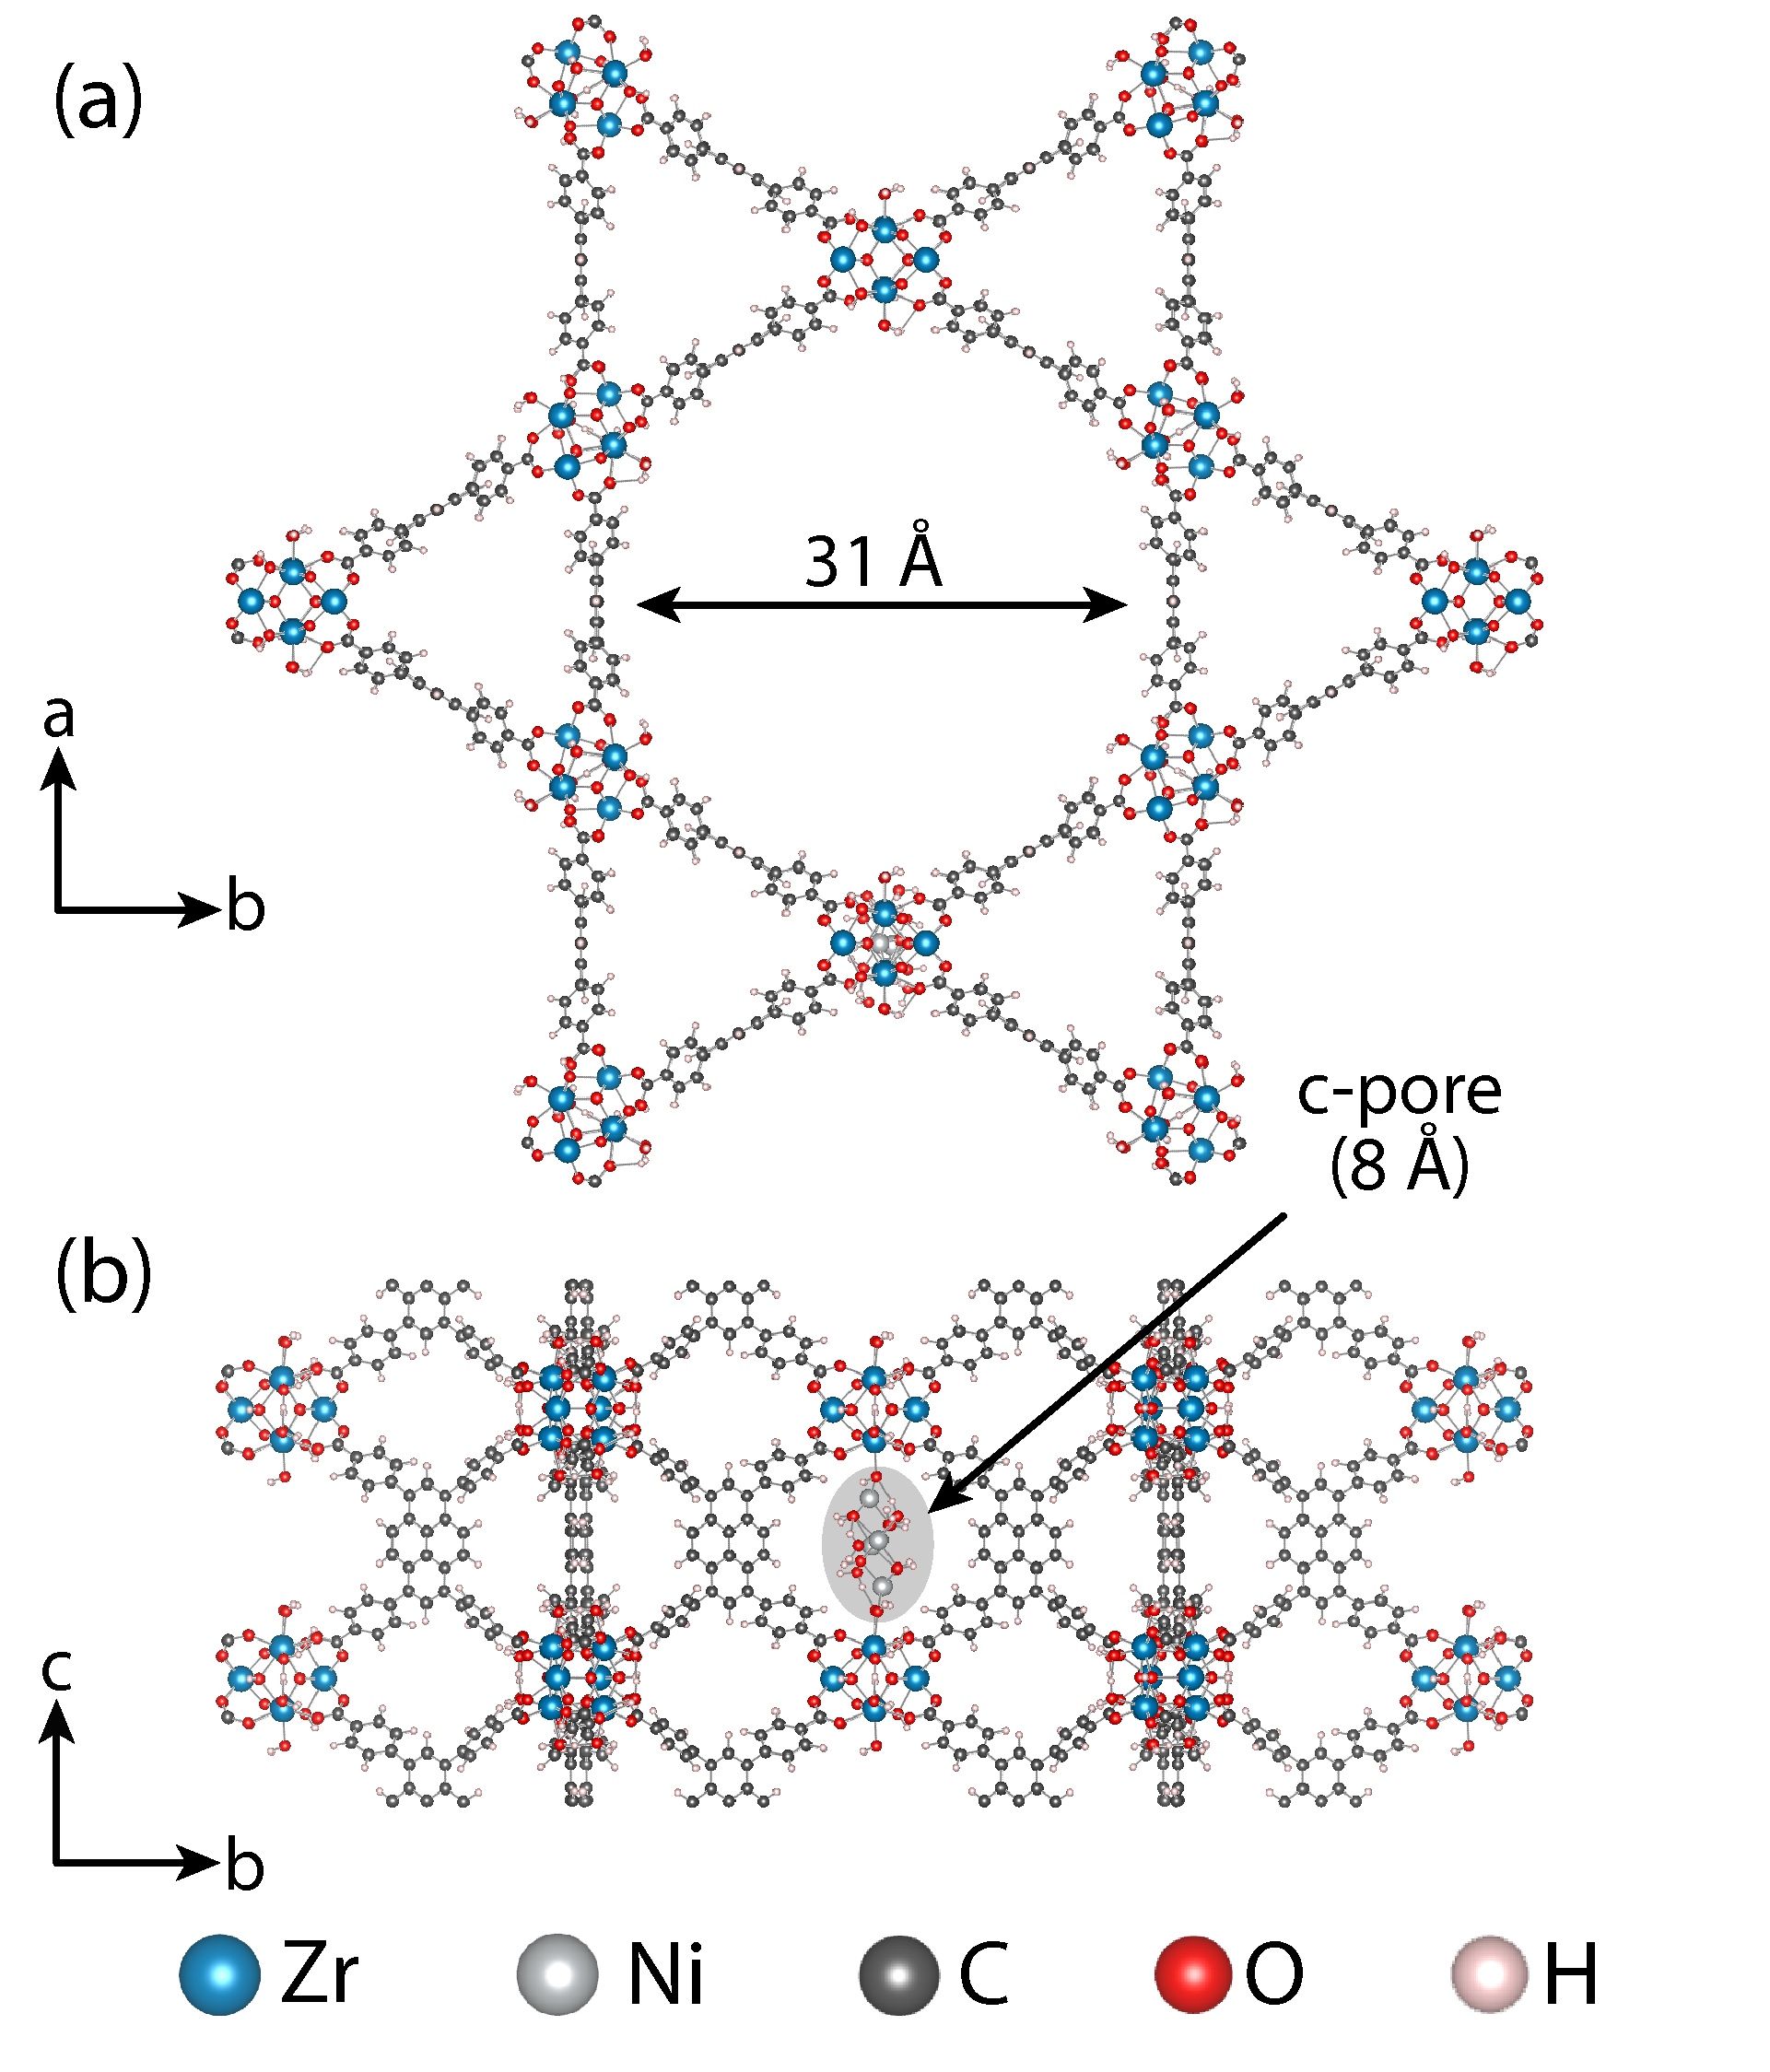
\includegraphics[width=3.0in]{zi-images/00-General-Graphics/2022-figure-MOF-schematic.png}
    \caption{
    The structure of NU-1000 shown along (a) the c-axis and (b) the a-axis with the location of the \ce{Ni} metal cluster highlighted by the gray oval. 
    }
    \label{fig:Ni-MOF-model}
\end{figure}

\subsection{Pair Distribution Function (PDF) Analysis}
Powder X-ray diffraction (XRD) and total scattering data suitable for PDF analysis are collected on Ni-NU-1000 catalysts at 50 \degree C in 3.5\% \ce{H2} (in \ce{He}) under ambient pressure, as described in a prior publication.\cite{PlateroPrats2017} The PDF provides structural information such as the distribution of interatomic distances in the Ni-NU-1000 catalysts and also reflects the \ce{Ni} coordination number and asymmetry in the \ce{Ni} coordination environment. PDFs represent the local structure as a histogram of atom-atom distances weighted by the scattering power of the atoms involved. Of interest are the \ce{Ni{\Compactcdots}Ni} and \ce{Ni-O} distances within the cluster and the \ce{Ni{\Compactcdots}Zr} distance between the cluster and NU-1000. In this notation, atom pairs not directly bonded to each other are denoted with ``${\Compactcdots}$". Given the lower scattering contribution from the \ce{O} atoms compared to \ce{Ni} atoms, \ce{O{\Compactcdots}O} pairs have very low contribution to the measured data and are not calculated. PDFs are calculated using the PDFgui software.\cite{Farrow2007}  To isolate the atom-atom distances that define the \ce{Ni} cluster and its interaction with NU-1000 support, d-PDFs are derived from PDFs by subtracting the PDF measured for NU-1000 from the PDF measured for Ni-NU-1000.

\subsection{Computational Details}

\subsubsection{Catalyst Structure Models}

Modeling is carried out to provide molecular level insight into the ligand environment of Ni-NU-1000. NU-1000 unit cells in the P6/mmm space group with DFT-optimized parameters of $a=b=40.611$ {\AA}, $c=15.990$ {\AA}, $\alpha=\beta=\ang{90}$, and $\gamma=\ang{60}$ are employed. \textcolor{red}{These periodic calculations are compared with their gas phase analogs in Supporting Information Section S1.11.} Following prior work,\cite{Ye2017} \ce{Ni} oxo catalysts are modeled with \ce{Ni4} clusters. Clusters comprising fewer than four \ce{Ni} ions were also evaluated, but gave poor agreement with the experimental d-PDF (see Supporting Information Section S3). \ce{Ni4} clusters span the 8 {\AA} pores of NU-1000, connecting two adjacent nodes (Figure~\ref{fig:Ni-MOF-model}b) by replacing a proton on each node.\cite{Ye2017} 

854 different ligand environments are considered to provide molecular-level insight into the types of ligand environments that could lead to the experimentally observed d-PDFs. These ligand environments include \ce{OH}, \ce{H2O}, \ce{O}, and \ce{H} and have stoichiometries of \ce{Ni_4O_xH_y}. Four example structures are shown in Figure~\ref{fig:Ni-MOF-structures}. The full library of structures considered in this work can be accessed on GitHub.\cite{GitHub-Ni4Project} \textcolor{red}{The GitHub repository also contains all input files required to replicate the DFT calculations of the most relevant structures identified in this work (i.e., CP2K input, pseudopotential, basis set, and dftb3 files), as well as the associated output files (i.e., output and frequency files).} \ce{Ni-O} coordination numbers are calculated for each structure according to geometric criteria (distance and orientation) as discussed in Supporting Information Section S1.7. 

\begin{figure}
    \centering
    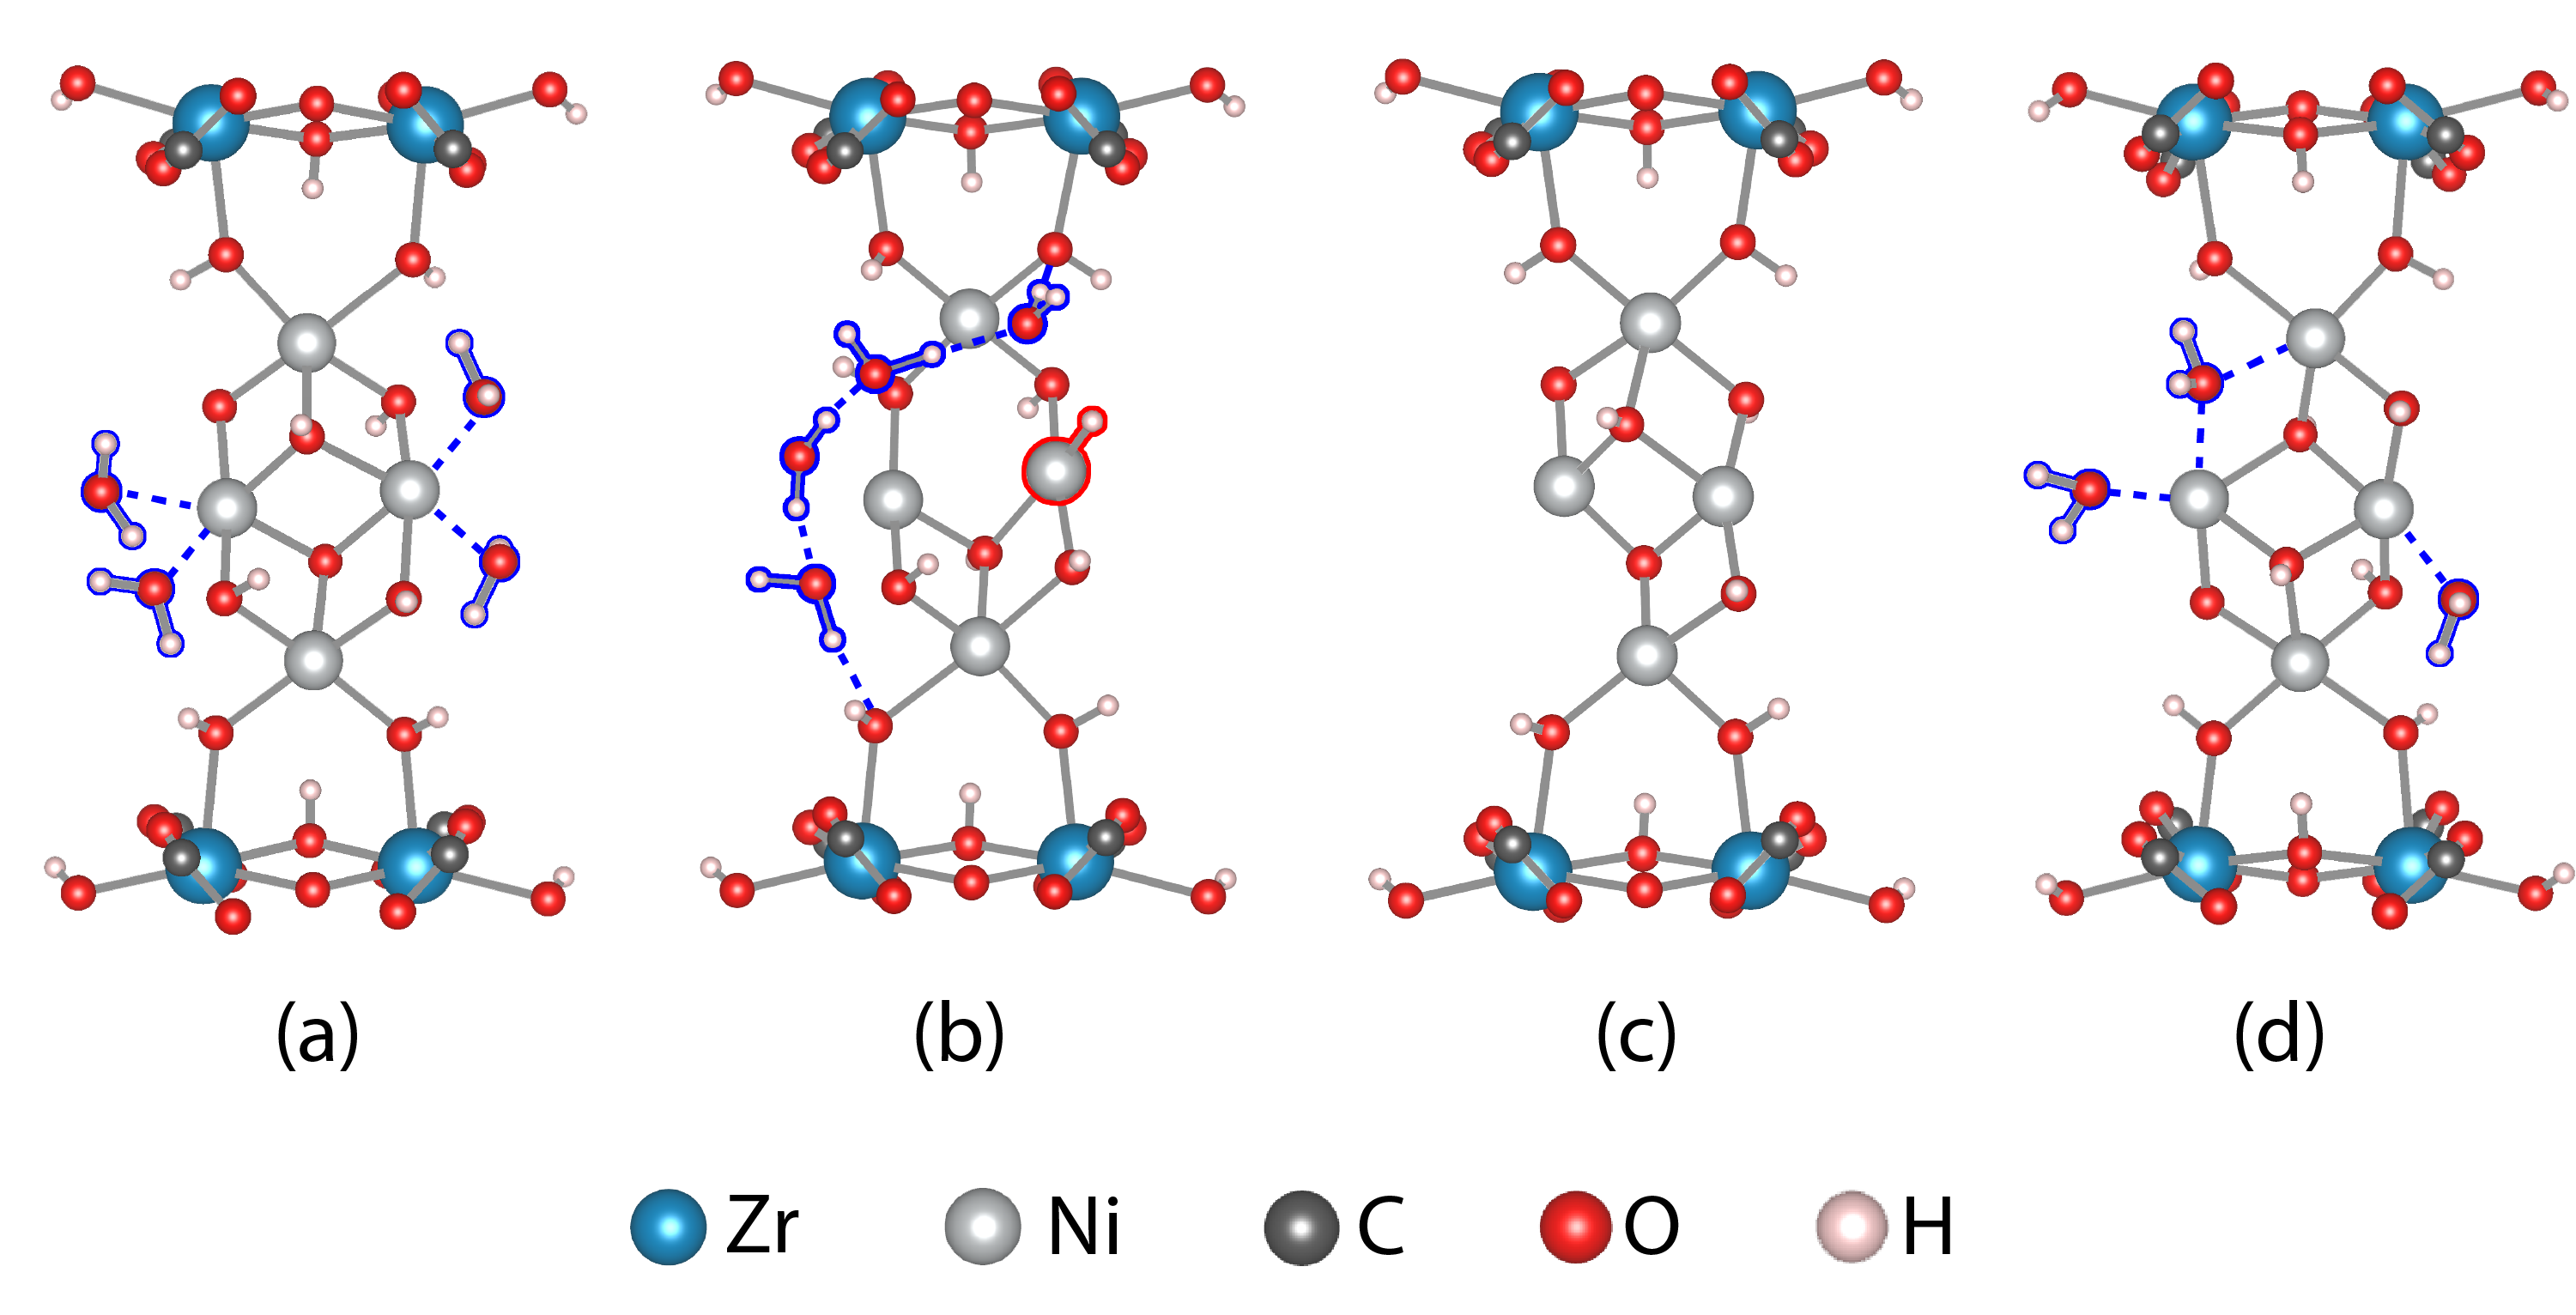
\includegraphics[width=5.0in]{zi-images/00-General-Graphics/2022-figure-clusters-3xstructures.png}
    \caption{
    Some of the \ce{Ni_4O_xH_y} clusters evaluated in this work. (a) \ce{Ni4(OH)6.4H2O} (green), (b) \ce{Ni4(OH)5(H).4H2O} (blue), (c) \ce{Ni4(OH)4(O)} (yellow), and (d) \ce{Ni4(OH)4(O).3H2O} (maroon). Colors in parentheses are the same as for Figures~\ref{fig:phase_diagram_Ni}, \ref{fig:Ni-structure-diagram}, and \ref{fig:dPDFs-graphic}. The NU-1000 structure is excluded from the pictures for clarity, except for the \ce{Zr} ions where the clusters are attached. \ce{H2O} and \ce{H} ligands are outlined in blue and red, respectively.
    }
    \label{fig:Ni-MOF-structures}
\end{figure}

\subsubsection{\textit{ab initio} Thermodynamics Modeling}

\textit{ab initio} thermodynamic analysis\cite{Reuter2003, Reuter2004, Grundner2015, Paolucci2016, Li2016, Getman2008, Mandal2020, Zuo2016, Tang2019} is used to identify the thermodynamically stable structures as functions of chemical potential ($\mu$, which can be related to gas phase temperature and partial pressure using an equation of state; see Supporting Information Section S1.3). Specifically, structure free energies are calculated as functions of  of $\mu_{\ce{H2}}$ and $\mu_{\ce{H2O}}$. \ce{H2} (g) is chosen since experimental d-PDFs are collected under hydrogenation conditions. \ce{H2O} (g) is chosen since we find hydrogen atom binding to the cluster often occurs on hydroxyl ligands, forming \ce{H2O} ligands, which can then desorb and because \ce{OH} and \ce{H2O} ligands are installed during AIM. \ce{H2O} (g) is hence a convenient oxygen reference (see Figure~S1). Cluster free energies are calculated as:
\begin{equation}
    \begin{split}
        \Delta F^{(2)}(V,T,\mu_{\text{H}},\mu_{\text{O}},N_{\text{Ni}})  
        & = \Delta F(V,T,N_{\text{H}},N_{\text{O}},N_{\text{Ni}}) - (\mu_{\text{H}})(\Delta N_{\text{H}}) \\
        & - (\mu_{\text{O}})(\Delta N_{\text{O}})  \\ 
    \end{split}
    \label{eq:free-energy-trans}
\end{equation}
where $F^{(2)}$ is the the second Legendre transform of the Helmholtz free energy (i.e., of $N_{\ce{H}}$ and $N_{\ce{O}}$ to $\mu_{\ce{H}}$ and $\mu_{\ce{O}}$),\cite{Alberty1997} $V$ is volume, $T$ is temperature, $\mu$ is chemical potential, and $N$ is number, i.e., of \ce{O} and \ce{H} atoms within the cluster. The $\Delta$'s in Eq.~\ref{eq:free-energy-trans} indicate quantities taken relative to a reference structure; the reference structure used in this work is the \ce{Ni4(OH)6.4H2O} structure shown in Figure~\ref{fig:Ni-MOF-structures}a. Here $\mu_{\ce{H}} = \frac{1}{2} \mu_{\ce{H}_2}$, and $\mu_{\text{O}} = \mu_{\ce{H2O}} - 2\mu_{\ce{H}}$. $F = E^\text{elec} + E^\text{ZP} + F^\text{vib}$, where $E^\text{elec}$ is the electronic energy calculated with DFT, $E^\text{ZP}$ is the zero point vibrational energy, and $F^\text{vib}$ is the temperature dependent vibrational free energy. $E^\text{ZP}$ and $F^\text{vib}$ are calculated from the DFT-calculated vibrational modes. Vibrational modes are only calculated for structures within 100 kJ/mol of the lowest electronic-energy cluster at each unique composition to decrease computational expense. Details about how the vibrational modes, $E^\text{ZP}$, and $F^\text{vib}$ are calculated are provided in Supporting Information Section S1.4.  

\subsubsection{Density Functional Theory Calculations}
Electronic energies are calculated using the CP2K software package\cite{Hutter2014} using the PBE exchange and correlation functional\cite{Perdew1996}, damped D3 dispersion corrections,\cite{Grimme2010} the DZVP-MOLOPT basis set,\cite{VandeVondele2007} and Goedecker pseudopotentials.\cite{Goedecker1996} \textcolor{red}{Comparisons of this method with the DFT + U approach, which can be important for systems comprising \ce{NiO} and \ce{NiOOH}, are made in Supporting Information Section S11.} Plane waves are simulated up to 360 Ry. As a single \ce{Ni} ion can adopt singlet or triplet spin states, we evaluate singlet, triplet, quintet, septet, and nonet states for the \ce{Ni4} clusters, following prior work.\cite{Shabbir2020, Ye2017, Bernales2016} The unrestricted Kohn-Sham (UKS) method is employed given the open shell nature of the system. Spin states exhibiting spin contamination are not considered in \textit{ab initio} thermodynamic analysis. Details about how spin contamination is determined and the criteria used to keep or discard structures is provided in Supporting Information Section S1.6. Electronic energies are obtained from geometry relaxations where the cell shape and volume are held fixed, but all atoms within the unit cell are allowed to relax. \textcolor{red}{We find a maximum 6~kJ/mol difference in the calculated electronic energies when the cell volume is allowed to relax also (see Supporting Information Section S12). As relaxation of the cell volume can have subtle influences on the structural details of the Ni clusters (see Supporting Information Section S12), structures are re-relaxed, this time allowing both the unit cell volume and atomic positions to relax, in order to create d-PDFs. Thermal fluctuations, which would impact the peak widths of the d-PDFs,\cite{PlateroPrats2016} are not included.} Other details about the DFT calculations, including how $E_{\text{H}_2}$ and $E_{\text{H}_2\text{O}}$ are calculated and sample CP2K input files for all types of DFT calculations carried out in this work are provided in Supporting Information Sections S1.8, S1.9, and S1.10.  

\section{Results}
%%%%%%%%%%%%%%%%%%%%%%%%%%%%%%%%%%%%%%%%%%%%%%%%%%%%%%%%%%%%%%%%%%%%%
%% Results 
%%%%%%%%%%%%%%%%%%%%%%%%%%%%%%%%%%%%%%%%%%%%%%%%%%%%%%%%%%%%%%%%%%%%%

\subsection{Comparison of \ce{Ni-O} Coordination Number and \ce{H2} Chemical Potential}

Results from \textit{ab initio} thermodynamic analysis are presented in Figure~\ref{fig:phase_diagram_Ni}, which is a phase diagram indicating the structures that minimize $\Delta F^{(2)}$ as a function of $\mu_{\ce{H}_2}$ and $\mu_{\ce{H2O}}$. The different colored regions correspond to different structures, which are depicted in Figure~\ref{fig:Ni-structure-diagram}a. \textcolor{red}{A combined phase diagram and structure diagram is provided in Supporting Information Section S10. Further, Supporting Information Section S9 illustrates the difference in free energy between the thermodynamic minimum structure and the next lowest free energy structure as a function of $\mu_{\ce{H}_2}$ and $\mu_{\ce{H2O}}$. Examples of such structures are provided in Supporting Information Section S8.}

% Phase Diagram
\begin{figure}[H]
    \centering
    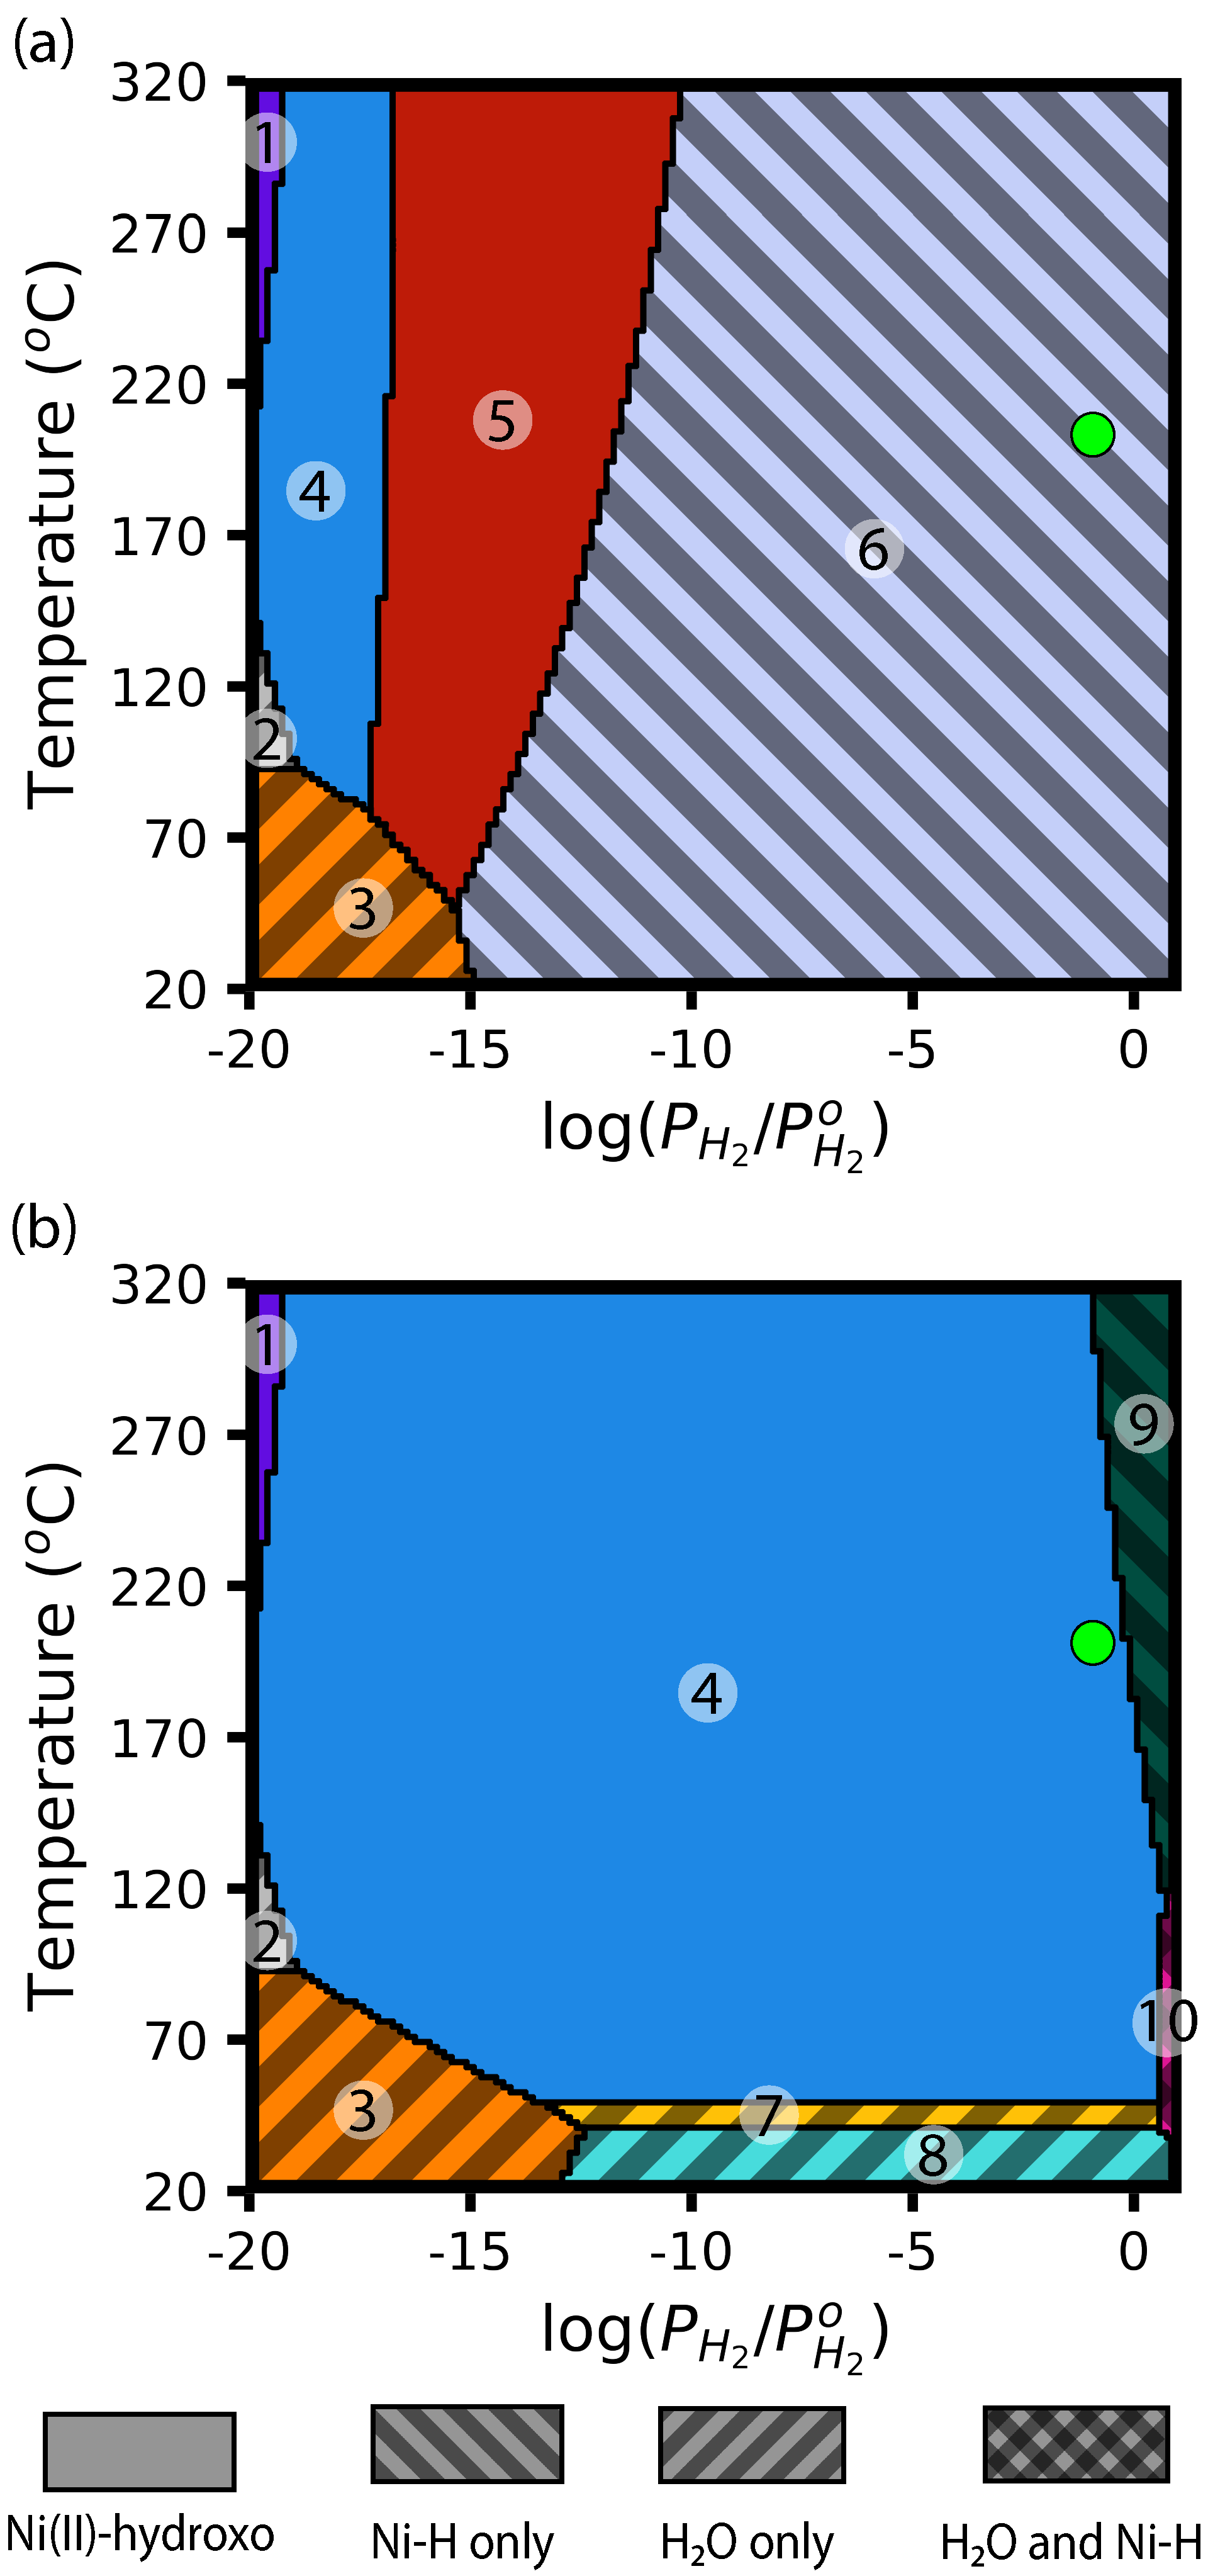
\includegraphics{zi-images/01-Ni-Graphics/2021-MAIN-phase-diagram-combined.png}
    \caption{
    Phase diagram calculated from \textit{ab initio} thermodynamic analysis presented as a function of $\Delta \mu_{\ce{H2}}$ and $\Delta \mu_{\ce{H2O}}$ ($\Delta$'s indicate values referenced to the 0~K values; see Supporting Information Section S1.5 for a derivation). The color code is the same key as in Figures~\ref{fig:Ni-structure-diagram} and \ref{fig:dPDFs-graphic}. Numbers are the associated \ce{Ni-O} coordination numbers. The vertical dashed line indicates the value of $\Delta \mu_{\text{H}_2}$ corresponding to the conditions where the experimental d-PDF was collected.\cite{PlateroPrats2016} 
    }
    \label{fig:phase_diagram_Ni}
\end{figure}  

% Structure Diagram
\begin{figure}
    \centering
    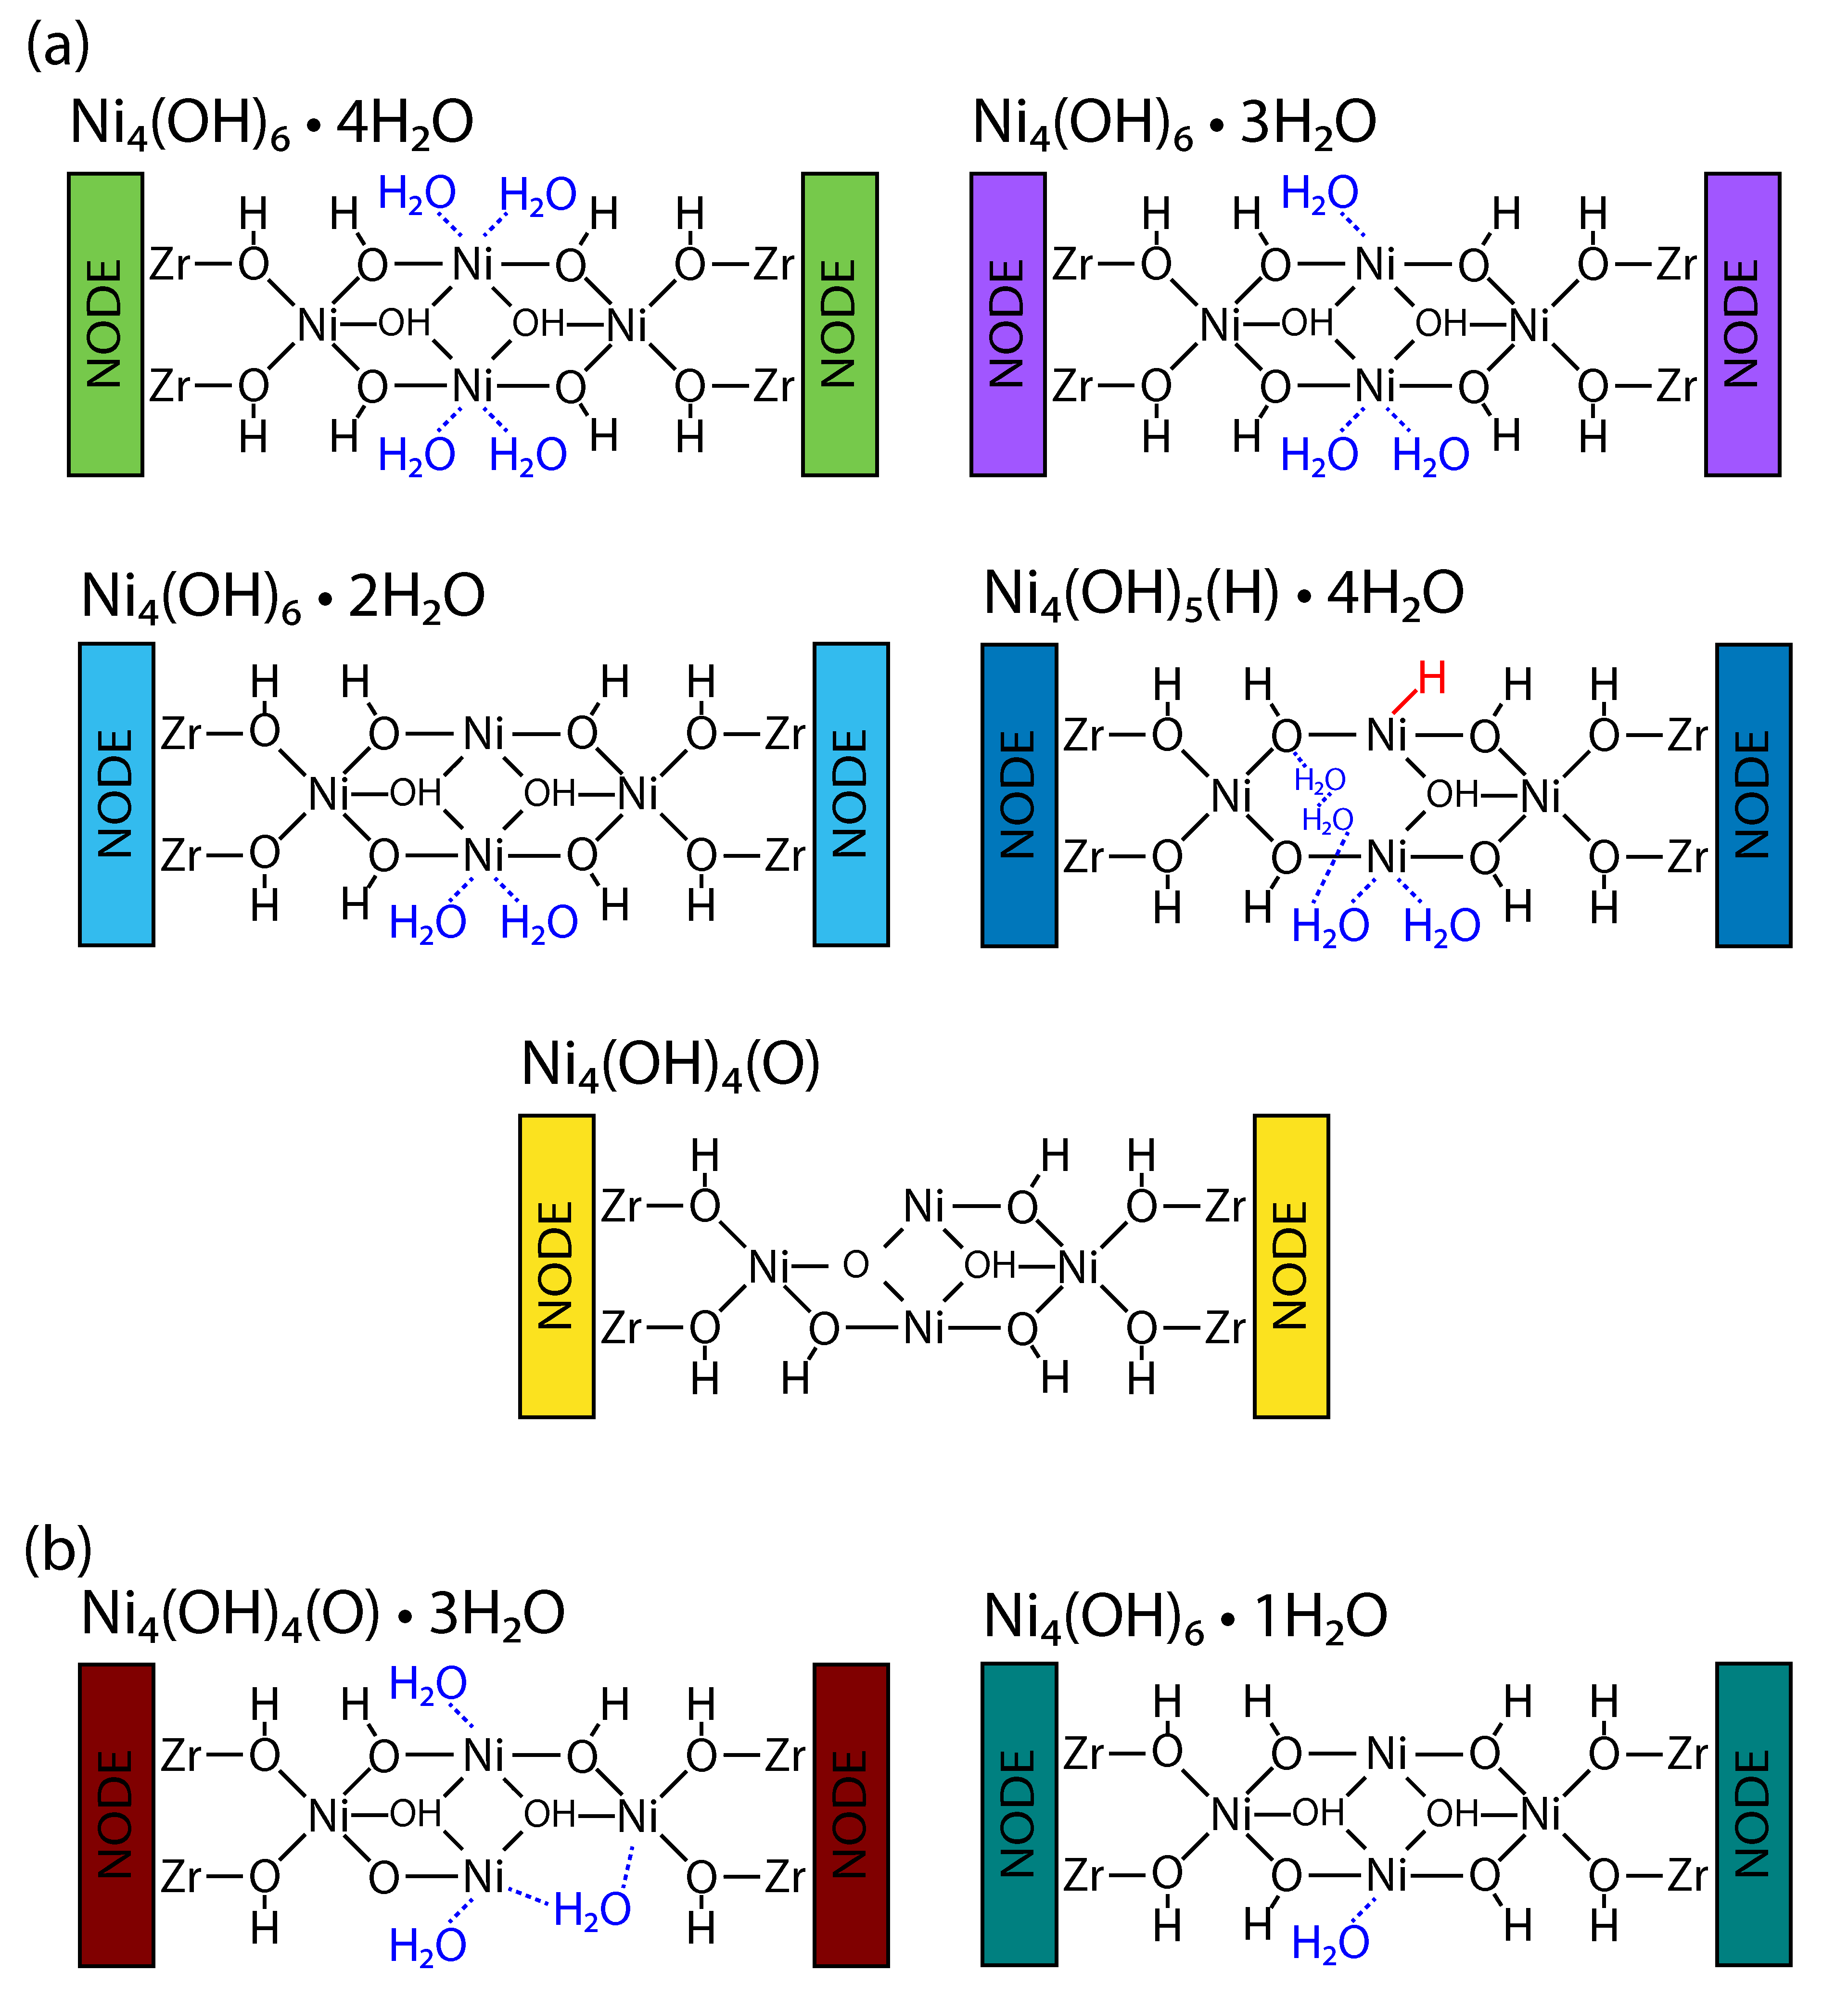
\includegraphics[width=0.75\textwidth]{zi-images/01-Ni-Graphics/2021-MAIN-structure-diagram.png}
    \caption{
    Depictions of (a) simulated thermodynamic minima structures with coordination numbers $\ge$ 4 and (b) simulated structures that are not thermodynamic minima but that exhibit broadening or splitting of the \ce{Ni{\Compactcdots}Ni} and/or \ce{Ni{\Compactcdots}Zr} peaks. \ce{H2O} molecules/ligands and \ce{H} ligands are indicated in blue and red text, respectively. Structure colors are the same as in Figures~\ref{fig:phase_diagram_Ni} and \ref{fig:dPDFs-graphic}: Part a: Top row: green (left), purple (right). Second row: cyan (left), blue (right). Third row: yellow. Part b: maroon (left), teal (right). 
    }
    \label{fig:Ni-structure-diagram}
\end{figure}

From Figure~\ref{fig:phase_diagram_Ni}, the \ce{Ni4(OH)6.4H2O} (green), \ce{Ni4(OH)5(H).4H2O} (blue), and \ce{Ni4(OH)4(O)} (yellow) structures are additionally shown in Figures~\ref{fig:Ni-MOF-structures}a-c. Prior work indicates that the average \ce{Ni-O} coordination number in the experimental structure is $\sim$5.\cite{PlateroPrats2017} Hence, in Figure~\ref{fig:phase_diagram_Ni}, each structure is annotated with its \ce{Ni-O} coordination number; ranges of $\mu_{\ce{H2}}$ and $\mu_{\ce{H2O}}$ are selected such that coordination numbers $\sim$5 are centered. The \ce{Ni4(OH)6.2H2O} (cyan), \ce{Ni4(OH)6.3H2O} (purple), and \ce{Ni4(OH)6.4H2O} (green) structures give \ce{Ni-O} coordination numbers of 5.0, 5.25, and 5.5, respectively, which are in line with the experimentally observed value of $\sim$5. These structures comprise significant \ce{OH} and \ce{H2O} ligands and no \ce{O} or \ce{H} ligands and are highly symmetric (Figure~\ref{fig:Ni-structure-diagram}a). They reside on the phase diagram at higher (more positive) values of $\mu_{\text{H}_2\text{O}}$ and lower (more negative) values of $\mu_{\text{H}_2}$. As the experimental d-PDF was obtained under hydrogenation conditions, this suggests that the \ce{H2O} is coming from NU-1000, reminiscent of the \ce{H2O} storage abilities of MOF-303 and MOF-801.\cite{Hanikel2021,Kim2017} \textcolor{red}{Hypothetically, this \ce{H2O} is left after AIM. For example, such \ce{H2O} molecules could bind to NU-1000 nodes during AIM and then later transfer to the Ni cluster. Test calculations (see Supporting Information S14) indicate that both processes are favorable for structures with \ce{Ni-O} coordination numbers just below 5. } 

The vertical dotted line in Figure~\ref{fig:phase_diagram_Ni} indicates values of $\mu_{\ce{H2}}$ used during collection of the experimental d-PDF. The \ce{Ni4(OH)6.3H2O} (purple) and \ce{Ni4(OH)5(H).4H2O} (blue) structures fall along this line. While the \ce{Ni-O} coordination number of the \ce{Ni4(OH)6.3H2O} (purple) structure is 5.25, the coordination number of the \ce{Ni4(OH)5(H).4H2O} (blue) structure is notably lower at 4.25.  From Figures~\ref{fig:Ni-MOF-structures}b and~\ref{fig:Ni-structure-diagram}a, the ligand environments on the different \ce{Ni} ions in the \ce{Ni4(OH)5(H).4H2O} (blue) structure are highly asymmetric, with one \ce{Ni} ion comprising four \ce{OH} ligands, one comprising five \ce{OH} ligands, one comprising \ce{OH} and \ce{H} ligands, and another comprising \ce{OH} and \ce{H2O} ligands, one of which is involved in a hydrogen bonded chain of \ce{H2O} molecules. \textcolor{red}{Interestingly, the \ce{Ni4(OH)5(H).4H2O} (blue) structure comprises a hydride ligand. Two other structures on the phase diagram, \ce{Ni4(OH)3(H).H2O} (magenta) and \ce{Ni4(H)4} (red), also comprise hydride ligands (see Supporting Information Section S5). These structures have even lower \ce{Ni-O} coordination numbers. Expansion of the phase diagram to higher and lower values of $\mu_{\text{H}_2}$ and $\mu_{\text{H}_2\text{O}}$ does not reveal any additional structures (or higher coordination numbers; see Supporting Information Section S4). These results suggest that, while hydride ligands are indeed stable under certain conditions, potentially including those under which the experimental d-PDF was collected, they exhibit \ce{Ni-O} coordination numbers that are too low to fully account for experimental observations.}   

\subsection{Comparison of \ce{Ni-O}, \ce{Ni{\Compactcdots}Ni}, and \ce{Ni{\Compactcdots}Zr} peaks}

% d-PDF Diagram
\begin{figure}
    \centering
    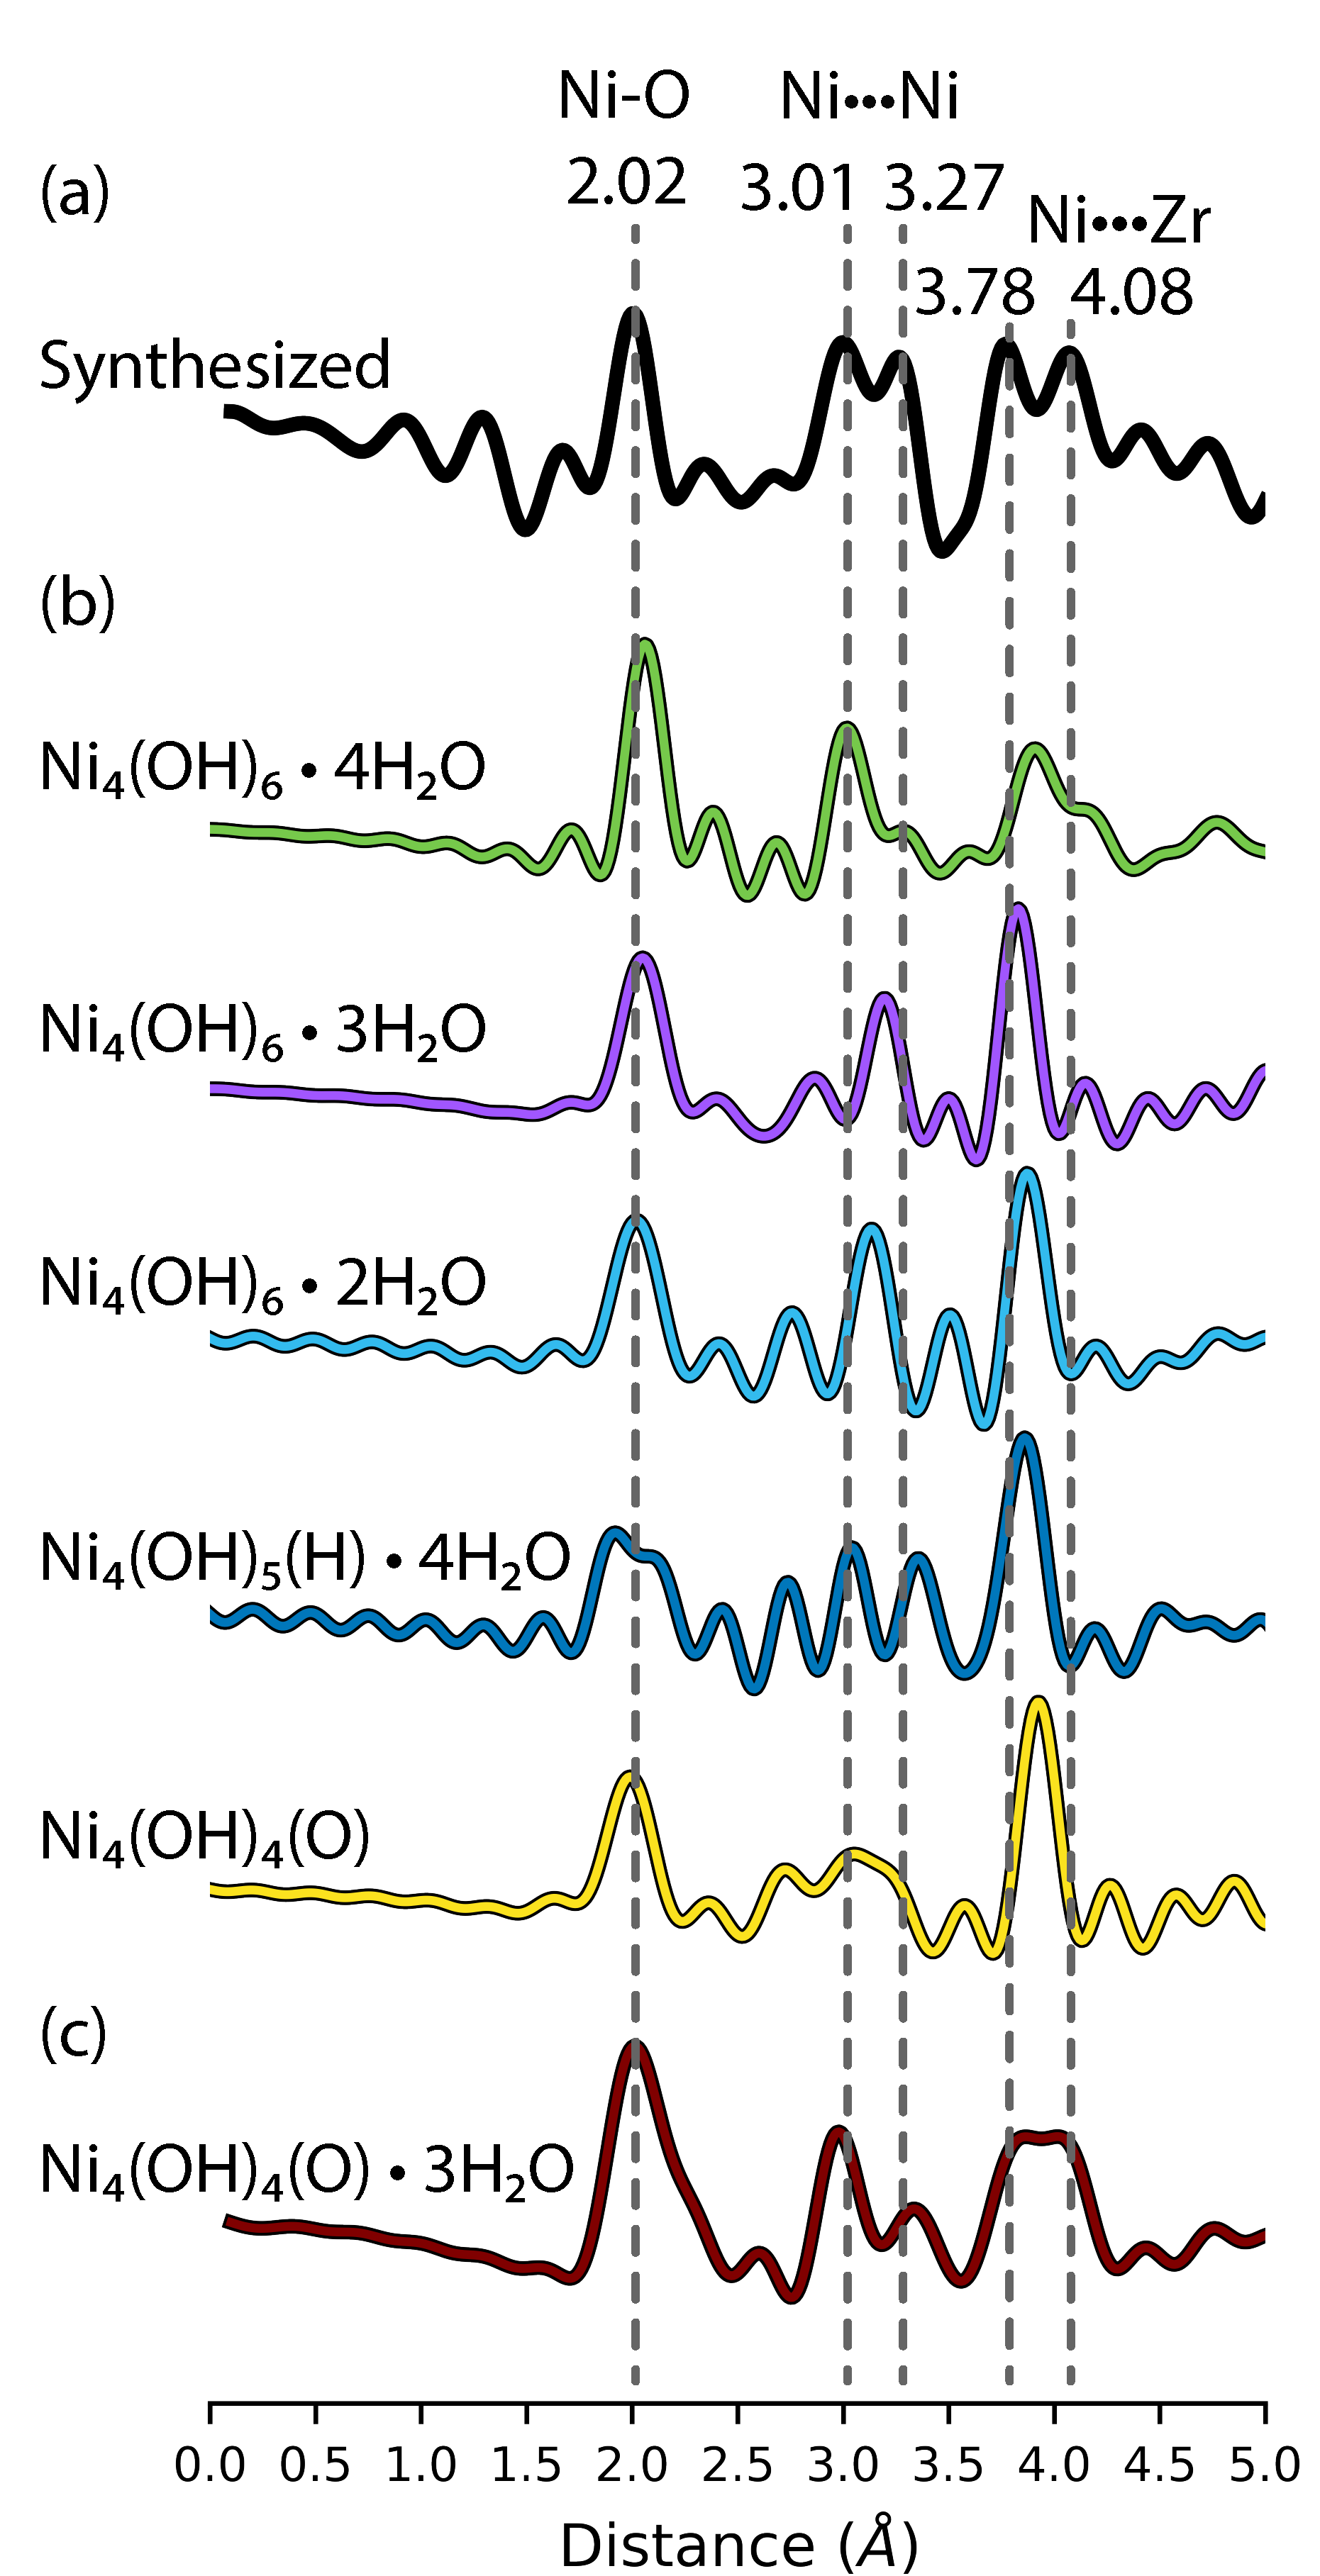
\includegraphics{zi-images/01-Ni-Graphics/2021-MAIN-single-dPDF.png}
    \caption{
    d-PDFs for (a) the synthesized structure, (b) the simulated thermodynamic minima structures with coordination numbers $\ge$ 4, (c) simulated structures that are not thermodynamic minima but that exhibit broadening or splitting of the \ce{Ni{\Compactcdots}Ni} and/or \ce{Ni{\Compactcdots}Zr} peaks, and (d) a distribution of structures constructed using Boltzmann-weighted free energies. Structure labels and colors for the simulated structures are the same as in Figures~\ref{fig:phase_diagram_Ni} and \ref{fig:Ni-structure-diagram}. Gray dotted lines = key distances in the synthesized structure. $\ast$ = \ce{Ni-O} peaks. $\ddagger$ = \ce{Ni{\Compactcdots}Ni} peaks. $\times$ = \ce{Ni{\Compactcdots}Zr} peaks.
    }
    \label{fig:dPDFs-graphic}
\end{figure}

The d-PDF for the synthesized Ni-NU-1000 catalyst is shown in Figure~\ref{fig:dPDFs-graphic}a.\cite{PlateroPrats2017} Key peaks are the single peak at 2.02 {\AA}, two ``split'' peaks at 3.01 {\AA} and 3.27 {\AA}, and two split peaks at 3.78 {\AA} and 4.08 {\AA}. These peaks correspond to \ce{Ni-O}, \ce{Ni{\Compactcdots}Ni}, and \ce{Ni{\Compactcdots}Zr} distances, respectively. The presence of multiple peaks describing one distance suggests asymmetry in the associated ligand environments. Here, splitting of the \ce{Ni{\Compactcdots}Ni} and \ce{Ni{\Compactcdots}Zr} peaks suggests some asymmetry in the ligand environments on Ni and Zr.

To compare with experiment, d-PDFs for all structures on the phase diagram with \ce{Ni-O} coordination numbers $\ge$ 4 are shown in Figure~\ref{fig:dPDFs-graphic}b. The \ce{Ni-O} peaks agree well with experiment, with all structures exhibiting just one \ce{Ni-O} peak at a distance of $\sim$2~\AA. There is less consistency in the \ce{Ni{\Compactcdots}Ni} peaks, with some structures exhibiting a single \ce{Ni{\Compactcdots}Ni} peak and others exhibiting multiple. The \ce{Ni4(OH)5(H).4H2O} (blue), \ce{Ni4(OH)6.2H2O} (cyan), and \ce{Ni4(OH)4(O)} (yellow) structures, which have varying degrees of asymmetry, exhibit multiple \ce{Ni{\Compactcdots}Ni} peaks.  Specifically, the \ce{Ni4(OH)5(H).4H2O} (blue) structure exhibits three \ce{Ni{\Compactcdots}Ni} peaks, i.e., more than observed experimentally, due to the highly asymmetric ligand environment. Alternatively, the \ce{Ni4(OH)6.2H2O} (cyan) and and \ce{Ni4(OH)4(O)} (yellow) structures both exhibit two peaks, in line with the experimental structure.  While the \ce{Ni-O} coordination number of the \ce{Ni4(OH)6.2H2O} (cyan) structure is in excellent agreement with experiment (both are $\sim$5), the \ce{Ni-O} coordination number of the \ce{Ni4(OH)4(O)} (yellow; Figures~\ref{fig:Ni-MOF-structures}c and~\ref{fig:Ni-structure-diagram}a) structure is significantly lower ($\sim$4). Further, this structure is stable at low $\mu_{\ce{H}_2}$, incommensurate with hydrogenation conditions and the conditions under which the experimental d-PDF was collected. The ligand environment in \ce{Ni4(OH)4(O)} (yellow) is hence unlikely to contribute to the observed d-PDF. On the other hand, the \ce{Ni4(OH)6.2H2O} (cyan) structure, which comprises \ce{OH} and \ce{H2O} ligands is feasible. This observation supports the suggestion from \ce{Ni-O} coordination number analysis that the experimental structure comprises significant \ce{OH} and \ce{H2O} ligands.

The last remaining feature of the d-PDFs is the \ce{Ni{\Compactcdots}Zr} peaks. Similar to the \ce{Ni{\Compactcdots}Ni} peaks, there is inconsistency within the \ce{Ni{\Compactcdots}Zr} peaks. Specifically, the  experimental d-PDF (Figure~\ref{fig:dPDFs-graphic}a) exhibits split peaks, while the simulated structures (Figure~\ref{fig:dPDFs-graphic}b) all exhibit a single peak. As none of the d-PDFs in Figure~\ref{fig:dPDFs-graphic}b exhibit split \ce{Ni{\Compactcdots}Zr} peaks, we generated d-PDFs for additional structures in order to learn the ligand environments that could induce splitting of the \ce{Ni{\Compactcdots}Zr} peaks. Specifically, we generated d-PDFs for the remaining simulated structures in the original dataset of 854. We found none that exhibits split \ce{Ni{\Compactcdots}Zr} peaks; however, one structure, \ce{Ni4(OH)4(O).3H2O} (maroon; Figures~\ref{fig:Ni-MOF-structures}d and \ref{fig:Ni-structure-diagram}b), exhibits a broad \ce{Ni{\Compactcdots}Zr} peak (Figure~\ref{fig:dPDFs-graphic}c). This structure comprises an asymmetric mixture of \ce{OH}, \ce{H2O}, and \ce{O} ligands, including one \ce{H2O} molecule that bridges a terminal \ce{Ni} ion with an adjacent bridging \ce{Ni} ion, analogous to the \ce{\mu_{2}-OH} ligands seen in the other structures in Figure~\ref{fig:Ni-structure-diagram}a. The \ce{Ni4(OH)4(O).3H2O} (maroon) structure is at least $\sim$350~kJ/mol higher in free energy than any structure on the phase diagram (see Supporting Information Figure~S19b), making it unlikely that the ligand environment in the experimental structure follows that of \ce{Ni4(OH)4(O).3H2O} (maroon). However, similarities between the \ce{Ni4(OH)4(O).3H2O} (maroon) d-PDF and the experimental d-PDF suggest \ce{H2O} ligands, particularly that connect to terminal \ce{Ni} ions in the cluster, as possible reasons for \ce{Ni{\Compactcdots}Zr} peak splitting. An alternative explanation for \ce{Ni{\Compactcdots}Zr} peak splitting is node distortions, which have been previously observed for NU-1000 during \ce{Ni} deposition and under conditions relevant for catalytic hydrogenation.\cite{PlateroPrats2016} As this phenomenon was not taken into account in our models, it could explain why none of the simulated structures exhibit split \ce{Ni{\Compactcdots}Zr} peaks.  

\section{Discussion}
Our results suggest that the \ce{Ni} ions in \ce{Ni}-NU-1000 catalysts comprise \ce{OH}, \ce{H2O}, and possibly \ce{H} ligands and that asymmetries in the ligand environment lead to split \ce{Ni{\Compactcdots}Ni} peaks. At \ce{Ni-O} coordination numbers $\le$5, these asymmetries may be as simple as different numbers of \ce{H2O} ligands on the different \ce{Ni} ions. To illustrate this, we computed the d-PDF for the \ce{Ni4(OH)6.1H2O} (teal) structure (Figure~\ref{fig:dPDFs-graphic}c). This structure comprises just one \ce{H2O} ligand and the remainder \ce{OH} ligands (Figure~\ref{fig:Ni-structure-diagram}b) and has a \ce{Ni-O} coordination number of 4.75. Like the compositionally similar \ce{Ni4(OH)6.2H2O} (cyan) structure (\ce{Ni-O} coordination number = 5.0), the \ce{Ni4(OH)6.1H2O} (teal) structure exhibits split \ce{Ni{\Compactcdots}Ni} peaks. In contrast, the \ce{Ni4(OH)6.3H2O} (purple) and \ce{Ni4(OH)6.4H2O} (green) structures, which are also compositionally similar but have \ce{Ni-O} coordination numbers of 5.25 and 5.5, exhibit a single \ce{Ni{\Compactcdots}Ni} peak.   

\textcolor{red}{An alternative explanation for the observed \ce{Ni{\Compactcdots}Ni} peak splitting is that fluxionality is important for Ni-NU-1000 catalysts under catalytic hydrogenation conditions.\cite{Halder2020, Halder2020ensemble}} To test this hypothesis, we constructed a d-PDF with contributions from multiple simulated structures based on their Boltzmann weights calculated from their relative free energies evaluated at various $\mu_{\ce{H2}}$ and $\mu_{\ce{H2O}}$ (see Supporting Information Section S7). An example of such a d-PDF is provided in Figure~\ref{fig:dPDFs-graphic}d. The d-PDF of this structure was constructed using chemical potentials near the boundaries between the \ce{Ni4(OH)6.3H2O} (purple) and \ce{Ni4(OH)6.4H2O} (green) structures in Figure~\ref{fig:phase_diagram_Ni} (i.e., $\Delta \mu_{\ce{H2}}$ = $-$250 kJ/mol and $\Delta \mu_{\ce{H2O}}$ = 205 kJ/mol). This Boltzmann weighted d-PDF exhibits a broad \ce{Ni{\Compactcdots}Ni} peak, suggesting that a distribution of ligand environments with subtly different \ce{H2O} contents could lead to split, or at least broadened \ce{Ni{\Compactcdots}Ni} peaks, even at \ce{Ni-O} coordination numbers $>$5. 




\section{Conclusions}
%%%%%%%%%%%%%%%%%%%%%%%%%%%%%%%%%%%%%%%%%%%%%%%%%%%%%%%%%%%%%%%%%%%%%
%% Conclusions  
%%%%%%%%%%%%%%%%%%%%%%%%%%%%%%%%%%%%%%%%%%%%%%%%%%%%%%%%%%%%%%%%%%%%%

The ligand environment of a \ce{Ni} oxo catalyst supported in the MOF NU-1000 is explored using a combination of experiments and simulations. Prior results indicate that the \ce{Ni-O} coordination number is $\sim$5. We find that clusters that exhibit such high coordination comprise a significant number of \ce{OH} and \ce{H2O} ligands and are only achievable under appreciable \ce{H2O} chemical potential. Given that experiments were performed under hydrogenation conditions, this suggests that \ce{H2O} in the cluster comes from the NU-1000 support. \textcolor{red}{Hypothetically, this \ce{H2O} is added to NU-1000 during AIM and remains even after thermal pretreatment.} Comparisons of experimental and simulated \ce{Ni-O} coordination numbers, \ce{H2} chemical potentials, and d-PDFs suggest ligand environments comprise \ce{OH}, \ce{H2O}, \textcolor{red}{and possibly \ce{H} ligands}. Further, asymmetric distributions of ligands, either within the same cluster or amongst a distribution of clusters within NU-1000, cause \ce{Ni{\Compactcdots}Ni} and possibly \ce{Ni{\Compactcdots}Zr} peak splitting.      

Interestingly, we only identified one stable structure comprising a \ce{Ni} hydride, i.e., structure \ce{Ni4(OH)5(H).4H2O} (blue), with a \ce{H2} chemical potential commensurate with hydrogenation conditions and conditions under which the experimental d-PDF was collected. However, the \ce{Ni-O} coordination number for this structure is notably lower at 4.25 than the experimentally observed value of $\sim$5. Further, the highly asymmetric ligand environment on this structure leads to three \ce{Ni{\Compactcdots}Ni} peaks, which is more than observed experimentally. These results suggest that if structures with hydride ligands exist in the experimental structure, they are present in relatively low amounts compared to structures with \ce{OH} and \ce{H2O} ligands. Alternatively, hydrides may be transient in catalytic hydrogenation and oligomerization, as hypothesized by \citeauthor{Li2016sintering}, or the active site could involve \ce{O}/\ce{OH} or \ce{OH}/\ce{H2O} ligands rather than a hydride, as proposed by \citeauthor{Shabbir2020} Answering these questions is a topic of ongoing work.  
%%%%%%%%%%%%%%%%%%%%%%%%%%%%%%%%%%%%%%%%%%%%%%%%%%%%%%%%%%%%%%%%%%%%%
%% Author Contact Information
%%%%%%%%%%%%%%%%%%%%%%%%%%%%%%%%%%%%%%%%%%%%%%%%%%%%%%%%%%%%%%%%%%%%%
\section{Author Contact Information}
\textcolor{red}{
\textbf{Stephen P. Vicchio} - \textit{Department of Chemical and Biomolecular Engineering, Clemson University, Clemson, South Carolina 29634-0909, United States} 
}
\\
\textcolor{red}{
\textbf{Zhihengyu Chen} - \textit{Department of Chemistry, Stony Brook University, Stony Brook, New York, 11794, United States} 
}
\\
\textcolor{red}{
\textbf{Karena W. Chapman} - \textit{Department of Chemistry, Stony Brook University, Stony Brook, New York, 11794, United States} 
}
\\
\textcolor{red}{
\textbf{Rachel B. Getman} - \textit{Department of Chemical and Biomolecular Engineering, Clemson University, Clemson, South Carolina 29634-0909, United States} 
}

%%%%%%%%%%%%%%%%%%%%%%%%%%%%%%%%%%%%%%%%%%%%%%%%%%%%%%%%%%%%%%%%%%%%%
%% Conflict of Interest Statement
%%%%%%%%%%%%%%%%%%%%%%%%%%%%%%%%%%%%%%%%%%%%%%%%%%%%%%%%%%%%%%%%%%%%%
\section{Conflict of Interest}
The authors declare no competing interests. 

%%%%%%%%%%%%%%%%%%%%%%%%%%%%%%%%%%%%%%%%%%%%%%%%%%%%%%%%%%%%%%%%%%%%%
%% The "Acknowledgement" section can be given in all manuscript
%% classes.  This should be given within the "acknowledgement"
%% environment, which will make the correct section or running title.
%%%%%%%%%%%%%%%%%%%%%%%%%%%%%%%%%%%%%%%%%%%%%%%%%%%%%%%%%%%%%%%%%%%%%
\begin{acknowledgement}

This work was supported as part of the Inorganometallic Catalyst Design Center, an Energy Frontier Research Center funded by the US Department of Energy, Office of Science, Basic Energy Sciences, under award DE-SC0012702. SPV is also supported by a GAANN Fellowship (Award Number: P200A180076) from the United States Department of Education. SPV and RBG would like to acknowledge the Clemson Computing and Information Technology (CITI) Advanced Computing and Data Science (ACDS) group for the generous allotment of compute time on the Palmetto cluster.

\end{acknowledgement}

%%%%%%%%%%%%%%%%%%%%%%%%%%%%%%%%%%%%%%%%%%%%%%%%%%%%%%%%%%%%%%%%%%%%%
%% The same is true for Supporting Information, which should use the
%% suppinfo environment.
%%%%%%%%%%%%%%%%%%%%%%%%%%%%%%%%%%%%%%%%%%%%%%%%%%%%%%%%%%%%%%%%%%%%%
\begin{suppinfo}
Further details in the computational parameters, \textit{ab initio} thermodynamic analysis, additional dPDFs, and phase diagrams. 
\end{suppinfo}

%%%%%%%%%%%%%%%%%%%%%%%%%%%%%%%%%%%%%%%%%%%%%%%%%%%%%%%%%%%%%%%%%%%%%
%% The appropriate \bibliography command should be placed here.
%% Notice that the class file automatically sets \bibliographystyle
%% and also names the section correctly.
%%%%%%%%%%%%%%%%%%%%%%%%%%%%%%%%%%%%%%%%%%%%%%%%%%%%%%%%%%%%%%%%%%%%%
% \bibliography{zreferences}
\providecommand{\latin}[1]{#1}
\makeatletter
\providecommand{\doi}
  {\begingroup\let\do\@makeother\dospecials
  \catcode`\{=1 \catcode`\}=2 \doi@aux}
\providecommand{\doi@aux}[1]{\endgroup\texttt{#1}}
\makeatother
\providecommand*\mcitethebibliography{\thebibliography}
\csname @ifundefined\endcsname{endmcitethebibliography}
  {\let\endmcitethebibliography\endthebibliography}{}
\begin{mcitethebibliography}{69}
\providecommand*\natexlab[1]{#1}
\providecommand*\mciteSetBstSublistMode[1]{}
\providecommand*\mciteSetBstMaxWidthForm[2]{}
\providecommand*\mciteBstWouldAddEndPuncttrue
  {\def\EndOfBibitem{\unskip.}}
\providecommand*\mciteBstWouldAddEndPunctfalse
  {\let\EndOfBibitem\relax}
\providecommand*\mciteSetBstMidEndSepPunct[3]{}
\providecommand*\mciteSetBstSublistLabelBeginEnd[3]{}
\providecommand*\EndOfBibitem{}
\mciteSetBstSublistMode{f}
\mciteSetBstMaxWidthForm{subitem}{(\alph{mcitesubitemcount})}
\mciteSetBstSublistLabelBeginEnd
  {\mcitemaxwidthsubitemform\space}
  {\relax}
  {\relax}

\bibitem[Thomas \latin{et~al.}(2005)Thomas, Raja, and Lewis]{Thomas2005}
Thomas,~J.~M.; Raja,~R.; Lewis,~D.~W. Single-site heterogeneous catalysts.
  \emph{Angewandte Chemie - International Edition} \textbf{2005}, \emph{44},
  6456--6482\relax
\mciteBstWouldAddEndPuncttrue
\mciteSetBstMidEndSepPunct{\mcitedefaultmidpunct}
{\mcitedefaultendpunct}{\mcitedefaultseppunct}\relax
\EndOfBibitem
\bibitem[Qiao \latin{et~al.}(2011)Qiao, Wang, Yang, Allard, Jiang, Cui, Liu,
  Li, and Zhang]{Qiao2011}
Qiao,~B.; Wang,~A.; Yang,~X.; Allard,~L.~F.; Jiang,~Z.; Cui,~Y.; Liu,~J.;
  Li,~J.; Zhang,~T. Single-atom catalysis of CO oxidation using Pt1/FeOx.
  \emph{Nature Chemistry} \textbf{2011}, \emph{3}, 634--641\relax
\mciteBstWouldAddEndPuncttrue
\mciteSetBstMidEndSepPunct{\mcitedefaultmidpunct}
{\mcitedefaultendpunct}{\mcitedefaultseppunct}\relax
\EndOfBibitem
\bibitem[Cui \latin{et~al.}(2017)Cui, Junge, Dai, Kreyenschulte, Pohl, Wohlrab,
  Shi, Brückner, and Beller]{Cui2017}
Cui,~X.; Junge,~K.; Dai,~X.; Kreyenschulte,~C.; Pohl,~M.~M.; Wohlrab,~S.;
  Shi,~F.; Brückner,~A.; Beller,~M. Synthesis of Single Atom Based
  Heterogeneous Platinum Catalysts: High Selectivity and Activity for
  Hydrosilylation Reactions. \emph{ACS Central Science} \textbf{2017},
  \emph{3}, 580--585\relax
\mciteBstWouldAddEndPuncttrue
\mciteSetBstMidEndSepPunct{\mcitedefaultmidpunct}
{\mcitedefaultendpunct}{\mcitedefaultseppunct}\relax
\EndOfBibitem
\bibitem[Yang \latin{et~al.}(2013)Yang, Wang, Qiao, Li, Liu, and
  Zhang]{Yang2013}
Yang,~X.~F.; Wang,~A.; Qiao,~B.; Li,~J.; Liu,~J.; Zhang,~T. Single-atom
  catalysts: A new frontier in heterogeneous catalysis. \emph{Accounts of
  Chemical Research} \textbf{2013}, \emph{46}, 1740--1748\relax
\mciteBstWouldAddEndPuncttrue
\mciteSetBstMidEndSepPunct{\mcitedefaultmidpunct}
{\mcitedefaultendpunct}{\mcitedefaultseppunct}\relax
\EndOfBibitem
\bibitem[Hlatky(2000)]{Hlatky2000}
Hlatky,~G.~G. Heterogeneous single-site catalysts for olefin polymerization.
  \emph{Chemical Reviews} \textbf{2000}, \emph{100}, 1347--1376\relax
\mciteBstWouldAddEndPuncttrue
\mciteSetBstMidEndSepPunct{\mcitedefaultmidpunct}
{\mcitedefaultendpunct}{\mcitedefaultseppunct}\relax
\EndOfBibitem
\bibitem[Kaiser \latin{et~al.}(2020)Kaiser, Chen, Akl, Mitchell, and
  Pérez-Ramírez]{Kaiser2020}
Kaiser,~S.~K.; Chen,~Z.; Akl,~D.~F.; Mitchell,~S.; Pérez-Ramírez,~J.
  Single-Atom Catalysts across the Periodic Table. \emph{Chemical Reviews}
  \textbf{2020}, 11703--11809\relax
\mciteBstWouldAddEndPuncttrue
\mciteSetBstMidEndSepPunct{\mcitedefaultmidpunct}
{\mcitedefaultendpunct}{\mcitedefaultseppunct}\relax
\EndOfBibitem
\bibitem[Wasson \latin{et~al.}(2019)Wasson, Buru, Chen, Islamoglu, and
  Farha]{Wasson2019}
Wasson,~M.~C.; Buru,~C.~T.; Chen,~Z.; Islamoglu,~T.; Farha,~O.~K.
  Metal–organic frameworks: A tunable platform to access single-site
  heterogeneous catalysts. \emph{Applied Catalysis A: General} \textbf{2019},
  \emph{586}, 1--20\relax
\mciteBstWouldAddEndPuncttrue
\mciteSetBstMidEndSepPunct{\mcitedefaultmidpunct}
{\mcitedefaultendpunct}{\mcitedefaultseppunct}\relax
\EndOfBibitem
\bibitem[Zheng \latin{et~al.}(2019)Zheng, Ye, Ortuño, Fulton, Gutiérrez,
  Camaioni, Motkuri, Li, Webber, Mehdi, Browning, Penn, Farha, Hupp, Truhlar,
  Cramer, and Lercher]{Zheng2019}
Zheng,~J. \latin{et~al.}  Selective Methane Oxidation to Methanol on Cu-Oxo
  Dimers Stabilized by Zirconia Nodes of an NU-1000 Metal-Organic Framework.
  \emph{Journal of the American Chemical Society} \textbf{2019}, \emph{141},
  9292--9304\relax
\mciteBstWouldAddEndPuncttrue
\mciteSetBstMidEndSepPunct{\mcitedefaultmidpunct}
{\mcitedefaultendpunct}{\mcitedefaultseppunct}\relax
\EndOfBibitem
\bibitem[Abdel-Mageed \latin{et~al.}(2019)Abdel-Mageed, Rungtaweevoranit,
  Parlinska-Wojtan, Pei, Yaghi, and Behm]{AbdelMageed2019}
Abdel-Mageed,~A.~M.; Rungtaweevoranit,~B.; Parlinska-Wojtan,~M.; Pei,~X.;
  Yaghi,~O.~M.; Behm,~R.~J. Highly Active and Stable Single-Atom Cu Catalysts
  Supported by a Metal-Organic Framework. \emph{Journal of the American
  Chemical Society} \textbf{2019}, \emph{141}, 5201--5210\relax
\mciteBstWouldAddEndPuncttrue
\mciteSetBstMidEndSepPunct{\mcitedefaultmidpunct}
{\mcitedefaultendpunct}{\mcitedefaultseppunct}\relax
\EndOfBibitem
\bibitem[Huang \latin{et~al.}(2019)Huang, Dong, Sun, Xue, Ma, Zheng, Liu, Li,
  Zhou, Qiao, Song, Ma, Zhang, Lin, and Wang]{Huang2019}
Huang,~C.; Dong,~J.; Sun,~W.; Xue,~Z.; Ma,~J.; Zheng,~L.; Liu,~C.; Li,~X.;
  Zhou,~K.; Qiao,~X.; Song,~Q.; Ma,~W.; Zhang,~L.; Lin,~Z.; Wang,~T.
  Coordination mode engineering in stacked-nanosheet metal–organic frameworks
  to enhance catalytic reactivity and structural robustness. \emph{Nature
  Communications} \textbf{2019}, \emph{10}, 1--10\relax
\mciteBstWouldAddEndPuncttrue
\mciteSetBstMidEndSepPunct{\mcitedefaultmidpunct}
{\mcitedefaultendpunct}{\mcitedefaultseppunct}\relax
\EndOfBibitem
\bibitem[Zhong \latin{et~al.}(2019)Zhong, Sa, Li, He, Li, Bi, Zhuang, Yu, and
  Zou]{Zhong2019}
Zhong,~W.; Sa,~R.; Li,~L.; He,~Y.; Li,~L.; Bi,~J.; Zhuang,~Z.; Yu,~Y.; Zou,~Z.
  A Covalent Organic Framework Bearing Single Ni Sites as a Synergistic
  Photocatalyst for Selective Photoreduction of CO2 to CO. \emph{Journal of the
  American Chemical Society} \textbf{2019}, \emph{141}, 7615--7621\relax
\mciteBstWouldAddEndPuncttrue
\mciteSetBstMidEndSepPunct{\mcitedefaultmidpunct}
{\mcitedefaultendpunct}{\mcitedefaultseppunct}\relax
\EndOfBibitem
\bibitem[Romero-Muñiz \latin{et~al.}(2020)Romero-Muñiz, Mavrandonakis,
  Albacete, Vega, Briois, Zamora, and Platero-Prats]{Romero-Muniz2020}
Romero-Muñiz,~I.; Mavrandonakis,~A.; Albacete,~P.; Vega,~A.; Briois,~V.;
  Zamora,~F.; Platero-Prats,~A.~E. Unveiling the Local Structure of Palladium
  Loaded into Imine-Linked Layered Covalent Organic Frameworks for
  Cross-Coupling Catalysis. \emph{Angewandte Chemie - International Edition}
  \textbf{2020}, \emph{59}, 13013--13020\relax
\mciteBstWouldAddEndPuncttrue
\mciteSetBstMidEndSepPunct{\mcitedefaultmidpunct}
{\mcitedefaultendpunct}{\mcitedefaultseppunct}\relax
\EndOfBibitem
\bibitem[Mao \latin{et~al.}(2016)Mao, Wang, Wang, and Hu]{Mao2016}
Mao,~Y.; Wang,~Z.; Wang,~H.~F.; Hu,~P. Understanding Catalytic Reactions over
  Zeolites: A Density Functional Theory Study of Selective Catalytic Reduction
  of NOx by NH3 over Cu-SAPO-34. \emph{ACS Catalysis} \textbf{2016}, \emph{6},
  7882--7891\relax
\mciteBstWouldAddEndPuncttrue
\mciteSetBstMidEndSepPunct{\mcitedefaultmidpunct}
{\mcitedefaultendpunct}{\mcitedefaultseppunct}\relax
\EndOfBibitem
\bibitem[Kistler \latin{et~al.}(2014)Kistler, Chotigkrai, Xu, Enderle,
  Praserthdam, Chen, Browning, and Gates]{Kistler2014}
Kistler,~J.~D.; Chotigkrai,~N.; Xu,~P.; Enderle,~B.; Praserthdam,~P.;
  Chen,~C.~Y.; Browning,~N.~D.; Gates,~B.~C. A single-site platinum CO
  oxidation catalyst in zeolite KLTL: Microscopic and spectroscopic
  determination of the locations of the platinum atoms. \emph{Angewandte Chemie
  - International Edition} \textbf{2014}, \emph{53}, 8904--8907\relax
\mciteBstWouldAddEndPuncttrue
\mciteSetBstMidEndSepPunct{\mcitedefaultmidpunct}
{\mcitedefaultendpunct}{\mcitedefaultseppunct}\relax
\EndOfBibitem
\bibitem[Patel \latin{et~al.}(2019)Patel, Hannagan, Kress, Schilling, Çlnar,
  and Sykes]{Patel2019}
Patel,~D.~A.; Hannagan,~R.~T.; Kress,~P.~L.; Schilling,~A.~C.; Çlnar,~V.;
  Sykes,~E. C.~H. Atomic-Scale Surface Structure and CO Tolerance of NiCu
  Single-Atom Alloys. \emph{Journal of Physical Chemistry C} \textbf{2019},
  \emph{123}, 28142--28147\relax
\mciteBstWouldAddEndPuncttrue
\mciteSetBstMidEndSepPunct{\mcitedefaultmidpunct}
{\mcitedefaultendpunct}{\mcitedefaultseppunct}\relax
\EndOfBibitem
\bibitem[Pei \latin{et~al.}(2017)Pei, Liu, Yang, Zhang, Wang, Li, Wang, Wang,
  and Zhang]{Pei2017}
Pei,~G.~X.; Liu,~X.~Y.; Yang,~X.; Zhang,~L.; Wang,~A.; Li,~L.; Wang,~H.;
  Wang,~X.; Zhang,~T. Performance of Cu-Alloyed Pd Single-Atom Catalyst for
  Semihydrogenation of Acetylene under Simulated Front-End Conditions.
  \emph{ACS Catalysis} \textbf{2017}, \emph{7}, 1491--1500\relax
\mciteBstWouldAddEndPuncttrue
\mciteSetBstMidEndSepPunct{\mcitedefaultmidpunct}
{\mcitedefaultendpunct}{\mcitedefaultseppunct}\relax
\EndOfBibitem
\bibitem[Jiao \latin{et~al.}(2019)Jiao, Lin, Liu, Cheong, Zhang, Chen, Pan,
  Tang, Wu, Hung, Chen, Zheng, Lu, Yang, Xu, Xiao, Li, Wang, Peng, Chen, and
  Li]{Jiao2019}
Jiao,~J. \latin{et~al.}  Copper atom-pair catalyst anchored on alloy nanowires
  for selective and efficient electrochemical reduction of CO 2. \emph{Nature
  Chemistry} \textbf{2019}, \emph{11}, 222--228\relax
\mciteBstWouldAddEndPuncttrue
\mciteSetBstMidEndSepPunct{\mcitedefaultmidpunct}
{\mcitedefaultendpunct}{\mcitedefaultseppunct}\relax
\EndOfBibitem
\bibitem[Bo \latin{et~al.}(2019)Bo, Thornburg, Peng, Moreno, Nolan, Marks, and
  Notestein]{Bo2019}
Bo,~Z.; Thornburg,~N.~E.; Peng,~L.; Moreno,~J. J.~G.; Nolan,~M.; Marks,~L.~D.;
  Notestein,~J.~M. Direct Visualization of Independent Ta Centers Supported on
  Two-Dimensional TiO2 Nanosheets. \emph{Nano Letters} \textbf{2019},
  \emph{19}, 8103--8108\relax
\mciteBstWouldAddEndPuncttrue
\mciteSetBstMidEndSepPunct{\mcitedefaultmidpunct}
{\mcitedefaultendpunct}{\mcitedefaultseppunct}\relax
\EndOfBibitem
\bibitem[Riley \latin{et~al.}(2018)Riley, Zhou, Kunwar, Riva, Peterson, Payne,
  Gao, Lin, Guo, and Datye]{Riley2018}
Riley,~C.; Zhou,~S.; Kunwar,~D.; Riva,~A. D.~L.; Peterson,~E.; Payne,~R.;
  Gao,~L.; Lin,~S.; Guo,~H.; Datye,~A. Design of Effective Catalysts for
  Selective Alkyne Hydrogenation by Doping of Ceria with a Single-Atom
  Promotor. \emph{Journal of the American Chemical Society} \textbf{2018},
  \emph{140}, 12964--12973\relax
\mciteBstWouldAddEndPuncttrue
\mciteSetBstMidEndSepPunct{\mcitedefaultmidpunct}
{\mcitedefaultendpunct}{\mcitedefaultseppunct}\relax
\EndOfBibitem
\bibitem[Tang \latin{et~al.}(2019)Tang, Asokan, Xu, Graham, Pan, Christopher,
  Li, and Sautet]{Tang2019}
Tang,~Y.; Asokan,~C.; Xu,~M.; Graham,~G.~W.; Pan,~X.; Christopher,~P.; Li,~J.;
  Sautet,~P. Rh single atoms on TiO2 dynamically respond to reaction conditions
  by adapting their site. \emph{Nature Communications} \textbf{2019},
  \emph{10}, 1--10\relax
\mciteBstWouldAddEndPuncttrue
\mciteSetBstMidEndSepPunct{\mcitedefaultmidpunct}
{\mcitedefaultendpunct}{\mcitedefaultseppunct}\relax
\EndOfBibitem
\bibitem[DeRita \latin{et~al.}(2019)DeRita, Resasco, Dai, Boubnov, Thang,
  Hoffman, Ro, Graham, Bare, Pacchioni, Pan, and Christopher]{DeRita2019}
DeRita,~L.; Resasco,~J.; Dai,~S.; Boubnov,~A.; Thang,~H.~V.; Hoffman,~A.~S.;
  Ro,~I.; Graham,~G.~W.; Bare,~S.~R.; Pacchioni,~G.; Pan,~X.; Christopher,~P.
  Structural evolution of atomically dispersed Pt catalysts dictates
  reactivity. \emph{Nature Materials} \textbf{2019}, \emph{18}, 746--751\relax
\mciteBstWouldAddEndPuncttrue
\mciteSetBstMidEndSepPunct{\mcitedefaultmidpunct}
{\mcitedefaultendpunct}{\mcitedefaultseppunct}\relax
\EndOfBibitem
\bibitem[Rogge \latin{et~al.}(2017)Rogge, Bavykina, Hajek, Garcia,
  Olivos-Suarez, Sepúlveda-Escribano, Vimont, Clet, Bazin, Kapteijn, Daturi,
  Ramos-Fernandez, Xamena, Speybroeck, and Gascon]{Rogge2017}
Rogge,~S.~M.; Bavykina,~A.; Hajek,~J.; Garcia,~H.; Olivos-Suarez,~A.~I.;
  Sepúlveda-Escribano,~A.; Vimont,~A.; Clet,~G.; Bazin,~P.; Kapteijn,~F.;
  Daturi,~M.; Ramos-Fernandez,~E.~V.; Xamena,~F. X.~L.; Speybroeck,~V.~V.;
  Gascon,~J. Metal-organic and covalent organic frameworks as single-site
  catalysts. \emph{Chemical Society Reviews} \textbf{2017}, \emph{46},
  3134--3184\relax
\mciteBstWouldAddEndPuncttrue
\mciteSetBstMidEndSepPunct{\mcitedefaultmidpunct}
{\mcitedefaultendpunct}{\mcitedefaultseppunct}\relax
\EndOfBibitem
\bibitem[Desai \latin{et~al.}(2018)Desai, Ye, Zheng, Ferrandon, Webber,
  Platero-Prats, Duan, Garcia-Holley, Camaioni, Chapman, Delferro, Farha,
  Fulton, Gagliardi, Lercher, Penn, Stein, and Lu]{Desai2018}
Desai,~S.~P. \latin{et~al.}  Well-Defined Rhodium-Gallium Catalytic Sites in a
  Metal-Organic Framework: Promoter-Controlled Selectivity in Alkyne
  Semihydrogenation to E-Alkenes. \emph{Journal of the American Chemical
  Society} \textbf{2018}, \emph{140}, 15309--15318\relax
\mciteBstWouldAddEndPuncttrue
\mciteSetBstMidEndSepPunct{\mcitedefaultmidpunct}
{\mcitedefaultendpunct}{\mcitedefaultseppunct}\relax
\EndOfBibitem
\bibitem[Manna \latin{et~al.}(2016)Manna, Ji, Lin, Greene, Urban, Thacker, and
  Lin]{Manna2016}
Manna,~K.; Ji,~P.; Lin,~Z.; Greene,~F.~X.; Urban,~A.; Thacker,~N.~C.; Lin,~W.
  Chemoselective single-site Earth-abundant metal catalysts at metal-organic
  framework nodes. \emph{Nature Communications} \textbf{2016}, \emph{7},
  1--11\relax
\mciteBstWouldAddEndPuncttrue
\mciteSetBstMidEndSepPunct{\mcitedefaultmidpunct}
{\mcitedefaultendpunct}{\mcitedefaultseppunct}\relax
\EndOfBibitem
\bibitem[Beyzavi \latin{et~al.}(2015)Beyzavi, Vermeulen, Howarth, Tussupbayev,
  League, Schweitzer, Gallagher, Platero-Prats, Hafezi, Sarjeant, Miller,
  Chapman, Stoddart, Cramer, Hupp, and Farha]{Beyzavi2015}
Beyzavi,~M.~H. \latin{et~al.}  A Hafnium-Based Metal-Organic Framework as a
  Nature-Inspired Tandem Reaction Catalyst. \emph{Journal of the American
  Chemical Society} \textbf{2015}, \emph{137}, 13624--13631\relax
\mciteBstWouldAddEndPuncttrue
\mciteSetBstMidEndSepPunct{\mcitedefaultmidpunct}
{\mcitedefaultendpunct}{\mcitedefaultseppunct}\relax
\EndOfBibitem
\bibitem[Shi \latin{et~al.}(2021)Shi, Lin, Luo, Wu, Li, Zhao, and
  Gong]{Shi2021}
Shi,~X.; Lin,~X.; Luo,~R.; Wu,~S.; Li,~L.; Zhao,~Z.-J.; Gong,~J. Dynamics of
  Heterogeneous Catalytic Processes at Operando Conditions. \emph{JACS Au}
  \textbf{2021}, \emph{1}, 2100--2120\relax
\mciteBstWouldAddEndPuncttrue
\mciteSetBstMidEndSepPunct{\mcitedefaultmidpunct}
{\mcitedefaultendpunct}{\mcitedefaultseppunct}\relax
\EndOfBibitem
\bibitem[Getman \latin{et~al.}(2008)Getman, Xu, and Schneider]{Getman2008}
Getman,~R.~B.; Xu,~Y.; Schneider,~W.~F. Thermodynamics of environment-dependent
  oxygen chemisorption on Pt(111). \emph{Journal of Physical Chemistry C}
  \textbf{2008}, \emph{112}, 9559--9572\relax
\mciteBstWouldAddEndPuncttrue
\mciteSetBstMidEndSepPunct{\mcitedefaultmidpunct}
{\mcitedefaultendpunct}{\mcitedefaultseppunct}\relax
\EndOfBibitem
\bibitem[Miller \latin{et~al.}(2011)Miller, Inoglu, and Kitchin]{Miller2011}
Miller,~S.~D.; Inoglu,~N.; Kitchin,~J.~R. Configurational correlations in the
  coverage dependent adsorption energies of oxygen atoms on late transition
  metal fcc(111) surfaces. \emph{Journal of Chemical Physics} \textbf{2011},
  \emph{134}, 1--8\relax
\mciteBstWouldAddEndPuncttrue
\mciteSetBstMidEndSepPunct{\mcitedefaultmidpunct}
{\mcitedefaultendpunct}{\mcitedefaultseppunct}\relax
\EndOfBibitem
\bibitem[Ranea \latin{et~al.}(2008)Ranea, Schneider, and Carmichael]{Ranea2008}
Ranea,~V.~A.; Schneider,~W.~F.; Carmichael,~I. DFT characterization of coverage
  dependent molecular water adsorption modes on α-Al2O3(0 0 0 1).
  \emph{Surface Science} \textbf{2008}, \emph{602}, 268--275\relax
\mciteBstWouldAddEndPuncttrue
\mciteSetBstMidEndSepPunct{\mcitedefaultmidpunct}
{\mcitedefaultendpunct}{\mcitedefaultseppunct}\relax
\EndOfBibitem
\bibitem[Heard \latin{et~al.}(2016)Heard, Siahrostami, and
  Grönbeck]{Heard2016}
Heard,~C.~J.; Siahrostami,~S.; Grönbeck,~H. Structural and Energetic Trends of
  Ethylene Hydrogenation over Transition Metal Surfaces. \emph{Journal of
  Physical Chemistry C} \textbf{2016}, \emph{120}, 995--1003\relax
\mciteBstWouldAddEndPuncttrue
\mciteSetBstMidEndSepPunct{\mcitedefaultmidpunct}
{\mcitedefaultendpunct}{\mcitedefaultseppunct}\relax
\EndOfBibitem
\bibitem[Bray and Schneider(2015)Bray, and Schneider]{Bray2014}
Bray,~J.~M.; Schneider,~W.~F. First-principles analysis of structure
  sensitivity in NO oxidation on Pt. \emph{ACS Catalysis} \textbf{2015},
  \emph{5}, 1087--1099\relax
\mciteBstWouldAddEndPuncttrue
\mciteSetBstMidEndSepPunct{\mcitedefaultmidpunct}
{\mcitedefaultendpunct}{\mcitedefaultseppunct}\relax
\EndOfBibitem
\bibitem[Gänzler \latin{et~al.}(2017)Gänzler, Casapu, Vernoux, Loridant,
  Aires, Epicier, Betz, Hoyer, and Grunwaldt]{Ganzler2017}
Gänzler,~A.~M.; Casapu,~M.; Vernoux,~P.; Loridant,~S.; Aires,~F. J. C.~S.;
  Epicier,~T.; Betz,~B.; Hoyer,~R.; Grunwaldt,~J.-D. Tuning the Structure of
  Platinum Particles on Ceria In Situ for Enhancing the Catalytic Performance
  of Exhaust Gas Catalysts. \emph{Angewandte Chemie} \textbf{2017}, \emph{129},
  13258--13262\relax
\mciteBstWouldAddEndPuncttrue
\mciteSetBstMidEndSepPunct{\mcitedefaultmidpunct}
{\mcitedefaultendpunct}{\mcitedefaultseppunct}\relax
\EndOfBibitem
\bibitem[Mandal \latin{et~al.}(2020)Mandal, Gu, Westendorff, Li, Pihl, Grabow,
  Epling, and Paolucci]{Mandal2020}
Mandal,~K.; Gu,~Y.; Westendorff,~K.~S.; Li,~S.; Pihl,~J.~A.; Grabow,~L.~C.;
  Epling,~W.~S.; Paolucci,~C. Condition-Dependent Pd Speciation and NO
  adsorption in Pd/Zeolites. \emph{ACS Catalysis} \textbf{2020},
  12801--12818\relax
\mciteBstWouldAddEndPuncttrue
\mciteSetBstMidEndSepPunct{\mcitedefaultmidpunct}
{\mcitedefaultendpunct}{\mcitedefaultseppunct}\relax
\EndOfBibitem
\bibitem[Felvey \latin{et~al.}(2022)Felvey, Guo, Rana, Xu, Bare, Gates, Katz,
  Kulkarni, Runnebaum, and Kronawitter]{Felvey2022}
Felvey,~N.; Guo,~J.; Rana,~R.; Xu,~L.; Bare,~S.~R.; Gates,~B.~C.; Katz,~A.;
  Kulkarni,~A.~R.; Runnebaum,~R.~C.; Kronawitter,~C.~X. Interconversion of
  Atomically Dispersed Platinum Cations and Platinum Clusters in Zeolite ZSM-5
  and Formation of Platinum gem-Dicarbonyls. \emph{Journal of the American
  Chemical Society} \textbf{2022}, \emph{144}, 13874--13887\relax
\mciteBstWouldAddEndPuncttrue
\mciteSetBstMidEndSepPunct{\mcitedefaultmidpunct}
{\mcitedefaultendpunct}{\mcitedefaultseppunct}\relax
\EndOfBibitem
\bibitem[Giewont \latin{et~al.}(2021)Giewont, Kyriakidou, and
  Walker]{Giewont2021}
Giewont,~K.; Kyriakidou,~E.~A.; Walker,~E.~A. Investigation of Potential
  Catalytic Active Sites of Pd/SSZ-13: A DFT Perspective. \emph{Journal of
  Physical Chemistry C} \textbf{2021}, \emph{125}, 15262--15274\relax
\mciteBstWouldAddEndPuncttrue
\mciteSetBstMidEndSepPunct{\mcitedefaultmidpunct}
{\mcitedefaultendpunct}{\mcitedefaultseppunct}\relax
\EndOfBibitem
\bibitem[Mesilov \latin{et~al.}(2021)Mesilov, Xiao, Dahlin, Bergman,
  Pettersson, and Bernasek]{Mesilov2021}
Mesilov,~V.; Xiao,~Y.; Dahlin,~S.; Bergman,~S.~L.; Pettersson,~L.~J.;
  Bernasek,~S.~L. First-Principles Calculations of Condition-Dependent Cu/Fe
  Speciation in Sulfur-Poisoned Cu- And Fe-SSZ-13 Catalysts. \emph{Journal of
  Physical Chemistry C} \textbf{2021}, \emph{125}, 4632--4645\relax
\mciteBstWouldAddEndPuncttrue
\mciteSetBstMidEndSepPunct{\mcitedefaultmidpunct}
{\mcitedefaultendpunct}{\mcitedefaultseppunct}\relax
\EndOfBibitem
\bibitem[Liu \latin{et~al.}(2019)Liu, Li, Zhang, Otake, Zhang, Peters, Young,
  Bedford, Letourneau, Mandia, Elam, Farha, and Hupp]{Liu2019}
Liu,~J.; Li,~Z.; Zhang,~X.; Otake,~K.~I.; Zhang,~L.; Peters,~A.~W.;
  Young,~M.~J.; Bedford,~N.~M.; Letourneau,~S.~P.; Mandia,~D.~J.; Elam,~J.~W.;
  Farha,~O.~K.; Hupp,~J.~T. Introducing Nonstructural Ligands to Zirconia-like
  Metal-Organic Framework Nodes to Tune the Activity of Node-Supported Nickel
  Catalysts for Ethylene Hydrogenation. \emph{ACS Catalysis} \textbf{2019},
  \emph{9}, 3198--3207\relax
\mciteBstWouldAddEndPuncttrue
\mciteSetBstMidEndSepPunct{\mcitedefaultmidpunct}
{\mcitedefaultendpunct}{\mcitedefaultseppunct}\relax
\EndOfBibitem
\bibitem[Reuben and Wittcoff(1988)Reuben, and Wittcoff]{1988Reuben}
Reuben,~B.; Wittcoff,~H. The SHOP process: An example of industrial creativity.
  \emph{Journal of Chemical Education} \textbf{1988}, \emph{65}, 605--607\relax
\mciteBstWouldAddEndPuncttrue
\mciteSetBstMidEndSepPunct{\mcitedefaultmidpunct}
{\mcitedefaultendpunct}{\mcitedefaultseppunct}\relax
\EndOfBibitem
\bibitem[Ross and Steel(1973)Ross, and Steel]{Ross1973}
Ross,~J. R.~H.; Steel,~M. C.~F. Mechanism of the steam reforming of methane
  over a coprecipitated nickel-alumina catalyst. \emph{J. Chem. Soc.{,} Faraday
  Trans. 1} \textbf{1973}, \emph{69}, 10--21\relax
\mciteBstWouldAddEndPuncttrue
\mciteSetBstMidEndSepPunct{\mcitedefaultmidpunct}
{\mcitedefaultendpunct}{\mcitedefaultseppunct}\relax
\EndOfBibitem
\bibitem[Ryabchuk \latin{et~al.}(2018)Ryabchuk, Agostini, Pohl, Lund, Agapova,
  Junge, Junge, and Beller]{Ryabchuk2018}
Ryabchuk,~P.; Agostini,~G.; Pohl,~M.-M.; Lund,~H.; Agapova,~A.; Junge,~H.;
  Junge,~K.; Beller,~M. Intermetallic nickel silicide nanocatalyst-A non-noble
  metal-based general hydrogenation catalyst. \emph{Science Advances}
  \textbf{2018}, \emph{4}, 1--10\relax
\mciteBstWouldAddEndPuncttrue
\mciteSetBstMidEndSepPunct{\mcitedefaultmidpunct}
{\mcitedefaultendpunct}{\mcitedefaultseppunct}\relax
\EndOfBibitem
\bibitem[Mondloch \latin{et~al.}(2013)Mondloch, Bury, Fairen-Jimenez, Kwon,
  Demarco, Weston, Sarjeant, Nguyen, Stair, Snurr, Farha, and
  Hupp]{Mondloch2013}
Mondloch,~J.~E.; Bury,~W.; Fairen-Jimenez,~D.; Kwon,~S.; Demarco,~E.~J.;
  Weston,~M.~H.; Sarjeant,~A.~A.; Nguyen,~S.~T.; Stair,~P.~C.; Snurr,~R.~Q.;
  Farha,~O.~K.; Hupp,~J.~T. Vapor-phase metalation by atomic layer deposition
  in a metal-organic framework. \emph{Journal of the American Chemical Society}
  \textbf{2013}, \emph{135}, 10294--10297\relax
\mciteBstWouldAddEndPuncttrue
\mciteSetBstMidEndSepPunct{\mcitedefaultmidpunct}
{\mcitedefaultendpunct}{\mcitedefaultseppunct}\relax
\EndOfBibitem
\bibitem[Li \latin{et~al.}(2016)Li, Schweitzer, League, Bernales, Peters,
  Getsoian, Wang, Miller, Vjunov, Fulton, Lercher, Cramer, Gagliardi, Hupp, and
  Farha]{Li2016sintering}
Li,~Z.; Schweitzer,~N.~M.; League,~A.~B.; Bernales,~V.; Peters,~A.~W.;
  Getsoian,~A.~B.; Wang,~T.~C.; Miller,~J.~T.; Vjunov,~A.; Fulton,~J.~L.;
  Lercher,~J.~A.; Cramer,~C.~J.; Gagliardi,~L.; Hupp,~J.~T.; Farha,~O.~K.
  Sintering-Resistant Single-Site Nickel Catalyst Supported by Metal-Organic
  Framework. \emph{Journal of the American Chemical Society} \textbf{2016},
  \emph{138}, 1977--1982\relax
\mciteBstWouldAddEndPuncttrue
\mciteSetBstMidEndSepPunct{\mcitedefaultmidpunct}
{\mcitedefaultendpunct}{\mcitedefaultseppunct}\relax
\EndOfBibitem
\bibitem[Platero-Prats \latin{et~al.}(2017)Platero-Prats, League, Bernales, Ye,
  Gallington, Vjunov, Schweitzer, Li, Zheng, Mehdi, Stevens, Dohnalkova,
  Balasubramanian, Farha, Hupp, Browning, Fulton, Camaioni, Lercher, Truhlar,
  Gagliardi, Cramer, and Chapman]{PlateroPrats2017}
Platero-Prats,~A.~E. \latin{et~al.}  Bridging Zirconia Nodes within a
  Metal-Organic Framework via Catalytic Ni-Hydroxo Clusters to Form
  Heterobimetallic Nanowires. \emph{Journal of the American Chemical Society}
  \textbf{2017}, \emph{139}, 10410--10418\relax
\mciteBstWouldAddEndPuncttrue
\mciteSetBstMidEndSepPunct{\mcitedefaultmidpunct}
{\mcitedefaultendpunct}{\mcitedefaultseppunct}\relax
\EndOfBibitem
\bibitem[Shabbir \latin{et~al.}(2020)Shabbir, Pellizzeri, Ferrandon, Kim,
  Vermeulen, Farha, Delferro, Martinson, and Getman]{Shabbir2020}
Shabbir,~H.; Pellizzeri,~S.; Ferrandon,~M.; Kim,~I.~S.; Vermeulen,~N.~A.;
  Farha,~O.~K.; Delferro,~M.; Martinson,~A.~B.; Getman,~R.~B. Influence of spin
  state and electron configuration on the active site and mechanism for
  catalytic hydrogenation on metal cation catalysts supported on NU-1000:
  insights from experiments and microkinetic modeling. \emph{Catalysis Science
  and Technology} \textbf{2020}, \emph{10}, 3594--3602\relax
\mciteBstWouldAddEndPuncttrue
\mciteSetBstMidEndSepPunct{\mcitedefaultmidpunct}
{\mcitedefaultendpunct}{\mcitedefaultseppunct}\relax
\EndOfBibitem
\bibitem[Yeh \latin{et~al.}(2021)Yeh, Vicchio, Chheda, Zheng, Schmid, Löbbert,
  Bermejo-Deval, Gutiérrez, Lercher, Lu, Neurock, Getman, Gagliardi, and
  Bhan]{Yeh2021}
Yeh,~B.; Vicchio,~S.~P.; Chheda,~S.; Zheng,~J.; Schmid,~J.; Löbbert,~L.;
  Bermejo-Deval,~R.; Gutiérrez,~O.~Y.; Lercher,~J.~A.; Lu,~C.~C.; Neurock,~M.;
  Getman,~R.~B.; Gagliardi,~L.; Bhan,~A. Site Densities, Rates, and Mechanism
  of Stable Ni/UiO-66 Ethylene Oligomerization Catalysts. \emph{Journal of the
  American Chemical Society} \textbf{2021}, \emph{143}, 20274--20280\relax
\mciteBstWouldAddEndPuncttrue
\mciteSetBstMidEndSepPunct{\mcitedefaultmidpunct}
{\mcitedefaultendpunct}{\mcitedefaultseppunct}\relax
\EndOfBibitem
\bibitem[Brogaard and Olsbye(2016)Brogaard, and Olsbye]{Brogaard2016}
Brogaard,~R.~Y.; Olsbye,~U. Ethene Oligomerization in Ni-Containing Zeolites:
  Theoretical Discrimination of Reaction Mechanisms. \emph{ACS Catalysis}
  \textbf{2016}, \emph{6}, 1205--1214\relax
\mciteBstWouldAddEndPuncttrue
\mciteSetBstMidEndSepPunct{\mcitedefaultmidpunct}
{\mcitedefaultendpunct}{\mcitedefaultseppunct}\relax
\EndOfBibitem
\bibitem[Wang \latin{et~al.}(2016)Wang, Vermeulen, Kim, Martinson, Stoddart,
  Hupp, and Farha]{Wang2016}
Wang,~T.~C.; Vermeulen,~N.~A.; Kim,~I.~S.; Martinson,~A.~B.; Stoddart,~J.~F.;
  Hupp,~J.~T.; Farha,~O.~K. Scalable synthesis and post-modification of a
  mesoporous metal-organic framework called NU-1000. \emph{Nature Protocols}
  \textbf{2016}, \emph{11}, 149--162\relax
\mciteBstWouldAddEndPuncttrue
\mciteSetBstMidEndSepPunct{\mcitedefaultmidpunct}
{\mcitedefaultendpunct}{\mcitedefaultseppunct}\relax
\EndOfBibitem
\bibitem[Ye \latin{et~al.}(2017)Ye, Gagliardi, Cramer, and Truhlar]{Ye2017}
Ye,~J.; Gagliardi,~L.; Cramer,~C.~J.; Truhlar,~D.~G. Single Ni atoms and Ni4
  clusters have similar catalytic activity for ethylene dimerization.
  \emph{Journal of Catalysis} \textbf{2017}, \emph{354}, 278--286\relax
\mciteBstWouldAddEndPuncttrue
\mciteSetBstMidEndSepPunct{\mcitedefaultmidpunct}
{\mcitedefaultendpunct}{\mcitedefaultseppunct}\relax
\EndOfBibitem
\bibitem[Farrow \latin{et~al.}(2007)Farrow, Juhas, Liu, Bryndin, Boin, Bloch,
  Proffen, and Billinge]{Farrow2007}
Farrow,~C.~L.; Juhas,~P.; Liu,~J.~W.; Bryndin,~D.; Boin,~E.~S.; Bloch,~J.;
  Proffen,~T.; Billinge,~S.~J. PDFfit2 and PDFgui: Computer programs for
  studying nanostructure in crystals. \emph{Journal of Physics Condensed
  Matter} \textbf{2007}, \emph{19}, 1--7\relax
\mciteBstWouldAddEndPuncttrue
\mciteSetBstMidEndSepPunct{\mcitedefaultmidpunct}
{\mcitedefaultendpunct}{\mcitedefaultseppunct}\relax
\EndOfBibitem
\bibitem[Platero-Prats \latin{et~al.}(2016)Platero-Prats, Mavrandonakis,
  Gallington, Liu, Hupp, Farha, Cramer, and Chapman]{PlateroPrats2016}
Platero-Prats,~A.~E.; Mavrandonakis,~A.; Gallington,~L.~C.; Liu,~Y.;
  Hupp,~J.~T.; Farha,~O.~K.; Cramer,~C.~J.; Chapman,~K.~W. Structural
  Transitions of the Metal-Oxide Nodes within Metal-Organic Frameworks: On the
  Local Structures of NU-1000 and UiO-66. \emph{Journal of the American
  Chemical Society} \textbf{2016}, \emph{138}, 4178--4185\relax
\mciteBstWouldAddEndPuncttrue
\mciteSetBstMidEndSepPunct{\mcitedefaultmidpunct}
{\mcitedefaultendpunct}{\mcitedefaultseppunct}\relax
\EndOfBibitem
\bibitem[Git(2022)]{GitHub-Ni4Project}
Ni4-Cluster-Structure-Files. 2022;
  \url{https://github.com/getman-research-group/Ni4-Cluster-Structure-Files}\relax
\mciteBstWouldAddEndPuncttrue
\mciteSetBstMidEndSepPunct{\mcitedefaultmidpunct}
{\mcitedefaultendpunct}{\mcitedefaultseppunct}\relax
\EndOfBibitem
\bibitem[Reuter and Scheffler(2003)Reuter, and Scheffler]{Reuter2003}
Reuter,~K.; Scheffler,~M. First-Principles Atomistic Thermodynamics for
  Oxidation Catalysis: Surface Phase Diagrams and Catalytically Interesting
  Regions. \emph{Physical Review Letters} \textbf{2003}, \emph{90}, 1--4\relax
\mciteBstWouldAddEndPuncttrue
\mciteSetBstMidEndSepPunct{\mcitedefaultmidpunct}
{\mcitedefaultendpunct}{\mcitedefaultseppunct}\relax
\EndOfBibitem
\bibitem[Reuter and Scheffler(2004)Reuter, and Scheffler]{Reuter2004}
Reuter,~K.; Scheffler,~M. Oxide formation at the surface of late 4d transition
  metals: Insights from first-principles atomistic thermodynamics.
  \emph{Applied Physics A: Materials Science and Processing} \textbf{2004},
  \emph{78}, 793--798\relax
\mciteBstWouldAddEndPuncttrue
\mciteSetBstMidEndSepPunct{\mcitedefaultmidpunct}
{\mcitedefaultendpunct}{\mcitedefaultseppunct}\relax
\EndOfBibitem
\bibitem[Grundner \latin{et~al.}(2015)Grundner, Markovits, Li, Tromp, Pidko,
  Hensen, Jentys, Sanchez-Sanchez, and Lercher]{Grundner2015}
Grundner,~S.; Markovits,~M.~A.; Li,~G.; Tromp,~M.; Pidko,~E.~A.; Hensen,~E.~J.;
  Jentys,~A.; Sanchez-Sanchez,~M.; Lercher,~J.~A. Single-site trinuclear copper
  oxygen clusters in mordenite for selective conversion of methane to methanol.
  \emph{Nature Communications} \textbf{2015}, \emph{6}, 1--9\relax
\mciteBstWouldAddEndPuncttrue
\mciteSetBstMidEndSepPunct{\mcitedefaultmidpunct}
{\mcitedefaultendpunct}{\mcitedefaultseppunct}\relax
\EndOfBibitem
\bibitem[Paolucci \latin{et~al.}(2016)Paolucci, Parekh, Khurana, Iorio, Li,
  Caballero, Shih, Anggara, Delgass, Miller, Ribeiro, Gounder, and
  Schneider]{Paolucci2016}
Paolucci,~C.; Parekh,~A.~A.; Khurana,~I.; Iorio,~J. R.~D.; Li,~H.;
  Caballero,~J. D.~A.; Shih,~A.~J.; Anggara,~T.; Delgass,~W.~N.; Miller,~J.~T.;
  Ribeiro,~F.~H.; Gounder,~R.; Schneider,~W.~F. Catalysis in a cage:
  Condition-dependent speciation and dynamics of exchanged cu cations in ssz-13
  zeolites. \emph{Journal of the American Chemical Society} \textbf{2016},
  \emph{138}, 6028--6048\relax
\mciteBstWouldAddEndPuncttrue
\mciteSetBstMidEndSepPunct{\mcitedefaultmidpunct}
{\mcitedefaultendpunct}{\mcitedefaultseppunct}\relax
\EndOfBibitem
\bibitem[Li \latin{et~al.}(2016)Li, Vassilev, Sanchez-Sanchez, Lercher, Hensen,
  and Pidko]{Li2016}
Li,~G.; Vassilev,~P.; Sanchez-Sanchez,~M.; Lercher,~J.~A.; Hensen,~E.~J.;
  Pidko,~E.~A. Stability and reactivity of copper oxo-clusters in ZSM-5 zeolite
  for selective methane oxidation to methanol. \emph{Journal of Catalysis}
  \textbf{2016}, \emph{338}, 305--312\relax
\mciteBstWouldAddEndPuncttrue
\mciteSetBstMidEndSepPunct{\mcitedefaultmidpunct}
{\mcitedefaultendpunct}{\mcitedefaultseppunct}\relax
\EndOfBibitem
\bibitem[Zuo \latin{et~al.}(2016)Zuo, Li, Liu, Han, and Huang]{Zuo2016}
Zuo,~Z.~J.; Li,~N.; Liu,~S.~Z.; Han,~P.~D.; Huang,~W. Initial stages of
  oxidation for Cu-based catalysts using density functional theory.
  \emph{Applied Surface Science} \textbf{2016}, \emph{366}, 85--94\relax
\mciteBstWouldAddEndPuncttrue
\mciteSetBstMidEndSepPunct{\mcitedefaultmidpunct}
{\mcitedefaultendpunct}{\mcitedefaultseppunct}\relax
\EndOfBibitem
\bibitem[Alberty(1997)]{Alberty1997}
Alberty,~R.~A. Legendre transforms in chemical thermodynamics. \emph{Journal of
  Chemical Thermodynamics} \textbf{1997}, \emph{29}, 501--516\relax
\mciteBstWouldAddEndPuncttrue
\mciteSetBstMidEndSepPunct{\mcitedefaultmidpunct}
{\mcitedefaultendpunct}{\mcitedefaultseppunct}\relax
\EndOfBibitem
\bibitem[Hutter \latin{et~al.}(2014)Hutter, Iannuzzi, Schiffmann, and
  Vandevondele]{Hutter2014}
Hutter,~J.; Iannuzzi,~M.; Schiffmann,~F.; Vandevondele,~J. {Cp2k: Atomistic
  simulations of condensed matter systems}. \emph{Wiley Interdisciplinary
  Reviews: Computational Molecular Science} \textbf{2014}, \emph{4},
  15--25\relax
\mciteBstWouldAddEndPuncttrue
\mciteSetBstMidEndSepPunct{\mcitedefaultmidpunct}
{\mcitedefaultendpunct}{\mcitedefaultseppunct}\relax
\EndOfBibitem
\bibitem[Perdew \latin{et~al.}(1996)Perdew, Burke, and Ernzerhof]{Perdew1996}
Perdew,~J.~P.; Burke,~K.; Ernzerhof,~M. Generalized Gradient Approximation Made
  Simple. \emph{Physical Review Letters} \textbf{1996}, \emph{77},
  3865--3868\relax
\mciteBstWouldAddEndPuncttrue
\mciteSetBstMidEndSepPunct{\mcitedefaultmidpunct}
{\mcitedefaultendpunct}{\mcitedefaultseppunct}\relax
\EndOfBibitem
\bibitem[Grimme \latin{et~al.}(2010)Grimme, Antony, Ehrlich, and
  Krieg]{Grimme2010}
Grimme,~S.; Antony,~J.; Ehrlich,~S.; Krieg,~H. A consistent and accurate ab
  initio parametrization of density functional dispersion correction (DFT-D)
  for the 94 elements H-Pu. \emph{Journal of Chemical Physics} \textbf{2010},
  \emph{132}, 1--20\relax
\mciteBstWouldAddEndPuncttrue
\mciteSetBstMidEndSepPunct{\mcitedefaultmidpunct}
{\mcitedefaultendpunct}{\mcitedefaultseppunct}\relax
\EndOfBibitem
\bibitem[VandeVondele and Hutter(2007)VandeVondele, and
  Hutter]{VandeVondele2007}
VandeVondele,~J.; Hutter,~J. Gaussian basis sets for accurate calculations on
  molecular systems in gas and condensed phases. \emph{Journal of Chemical
  Physics} \textbf{2007}, \emph{127}, 1--10\relax
\mciteBstWouldAddEndPuncttrue
\mciteSetBstMidEndSepPunct{\mcitedefaultmidpunct}
{\mcitedefaultendpunct}{\mcitedefaultseppunct}\relax
\EndOfBibitem
\bibitem[Goedecker \latin{et~al.}(1996)Goedecker, Teter, and
  Hutter]{Goedecker1996}
Goedecker,~S.; Teter,~M.; Hutter,~J. Separable dual-space Gaussian
  pseudopotentials. \emph{Physical Review B} \textbf{1996}, \emph{54},
  1703--1710\relax
\mciteBstWouldAddEndPuncttrue
\mciteSetBstMidEndSepPunct{\mcitedefaultmidpunct}
{\mcitedefaultendpunct}{\mcitedefaultseppunct}\relax
\EndOfBibitem
\bibitem[Bernales \latin{et~al.}(2016)Bernales, League, Li, Schweitzer, Peters,
  Carlson, Hupp, Cramer, Farha, and Gagliardi]{Bernales2016}
Bernales,~V.; League,~A.~B.; Li,~Z.; Schweitzer,~N.~M.; Peters,~A.~W.;
  Carlson,~R.~K.; Hupp,~J.~T.; Cramer,~C.~J.; Farha,~O.~K.; Gagliardi,~L.
  Computationally Guided Discovery of a Catalytic Cobalt-Decorated
  Metal-Organic Framework for Ethylene Dimerization. \emph{Journal of Physical
  Chemistry C} \textbf{2016}, \emph{120}, 23576--23583\relax
\mciteBstWouldAddEndPuncttrue
\mciteSetBstMidEndSepPunct{\mcitedefaultmidpunct}
{\mcitedefaultendpunct}{\mcitedefaultseppunct}\relax
\EndOfBibitem
\bibitem[Hanikel \latin{et~al.}(2021)Hanikel, Pei, Chheda, Lyu, Jeong, Sauer,
  Gagliardi, and Yaghi]{Hanikel2021}
Hanikel,~N.; Pei,~X.; Chheda,~S.; Lyu,~H.; Jeong,~W.; Sauer,~J.; Gagliardi,~L.;
  Yaghi,~O.~M. Evolution of water structures in metal-organic frameworks for
  improved atmospheric water harvesting. \emph{Science} \textbf{2021},
  \emph{374}, 454--459\relax
\mciteBstWouldAddEndPuncttrue
\mciteSetBstMidEndSepPunct{\mcitedefaultmidpunct}
{\mcitedefaultendpunct}{\mcitedefaultseppunct}\relax
\EndOfBibitem
\bibitem[Kim \latin{et~al.}(2017)Kim, Yang, Rao, Narayanan, Kapustin, Furukawa,
  Umans, Yaghi, and Wang]{Kim2017}
Kim,~H.; Yang,~S.; Rao,~S.~R.; Narayanan,~S.; Kapustin,~E.~A.; Furukawa,~H.;
  Umans,~A.~S.; Yaghi,~O.~M.; Wang,~E.~N. Water harvesting from air with
  metal-organic frameworks powered by natural sunlight. \emph{Science}
  \textbf{2017}, \emph{356}, 430--434\relax
\mciteBstWouldAddEndPuncttrue
\mciteSetBstMidEndSepPunct{\mcitedefaultmidpunct}
{\mcitedefaultendpunct}{\mcitedefaultseppunct}\relax
\EndOfBibitem
\bibitem[Halder \latin{et~al.}(2020)Halder, Lee, Yang, Pellin, Vajda, Li, Yang,
  Farha, and Hupp]{Halder2020}
Halder,~A.; Lee,~S.; Yang,~B.; Pellin,~M.~J.; Vajda,~S.; Li,~Z.; Yang,~Y.;
  Farha,~O.~K.; Hupp,~J.~T. Structural reversibility of Cu doped NU-1000 MOFs
  under hydrogenation conditions. \emph{Journal of Chemical Physics}
  \textbf{2020}, \emph{152}, 1--7\relax
\mciteBstWouldAddEndPuncttrue
\mciteSetBstMidEndSepPunct{\mcitedefaultmidpunct}
{\mcitedefaultendpunct}{\mcitedefaultseppunct}\relax
\EndOfBibitem
\bibitem[Halder \latin{et~al.}(2020)Halder, Ha, Zhai, Yang, Pellin, Seifert,
  Alexandrova, and Vajda]{Halder2020ensemble}
Halder,~A.; Ha,~M.~A.; Zhai,~H.; Yang,~B.; Pellin,~M.~J.; Seifert,~S.;
  Alexandrova,~A.~N.; Vajda,~S. Oxidative Dehydrogenation of Cyclohexane by Cu
  vs Pd Clusters: Selectivity Control by Specific Cluster Dynamics.
  \emph{ChemCatChem} \textbf{2020}, \emph{12}, 1307--1315\relax
\mciteBstWouldAddEndPuncttrue
\mciteSetBstMidEndSepPunct{\mcitedefaultmidpunct}
{\mcitedefaultendpunct}{\mcitedefaultseppunct}\relax
\EndOfBibitem
\end{mcitethebibliography}



%%%%%%%%%%%%%%%%%%%%%%%%%%%%%%%%%%%%%%%%%%%%%%%%%%%%%%%%%%%%%%%%%%%%%
%% 
%% Graphical TOC Entry
%%
%%%%%%%%%%%%%%%%%%%%%%%%%%%%%%%%%%%%%%%%%%%%%%%%%%%%%%%%%%%%%%%%%%%%%
\section{Graphical TOC Entry}
\begin{figure}
    \centering
    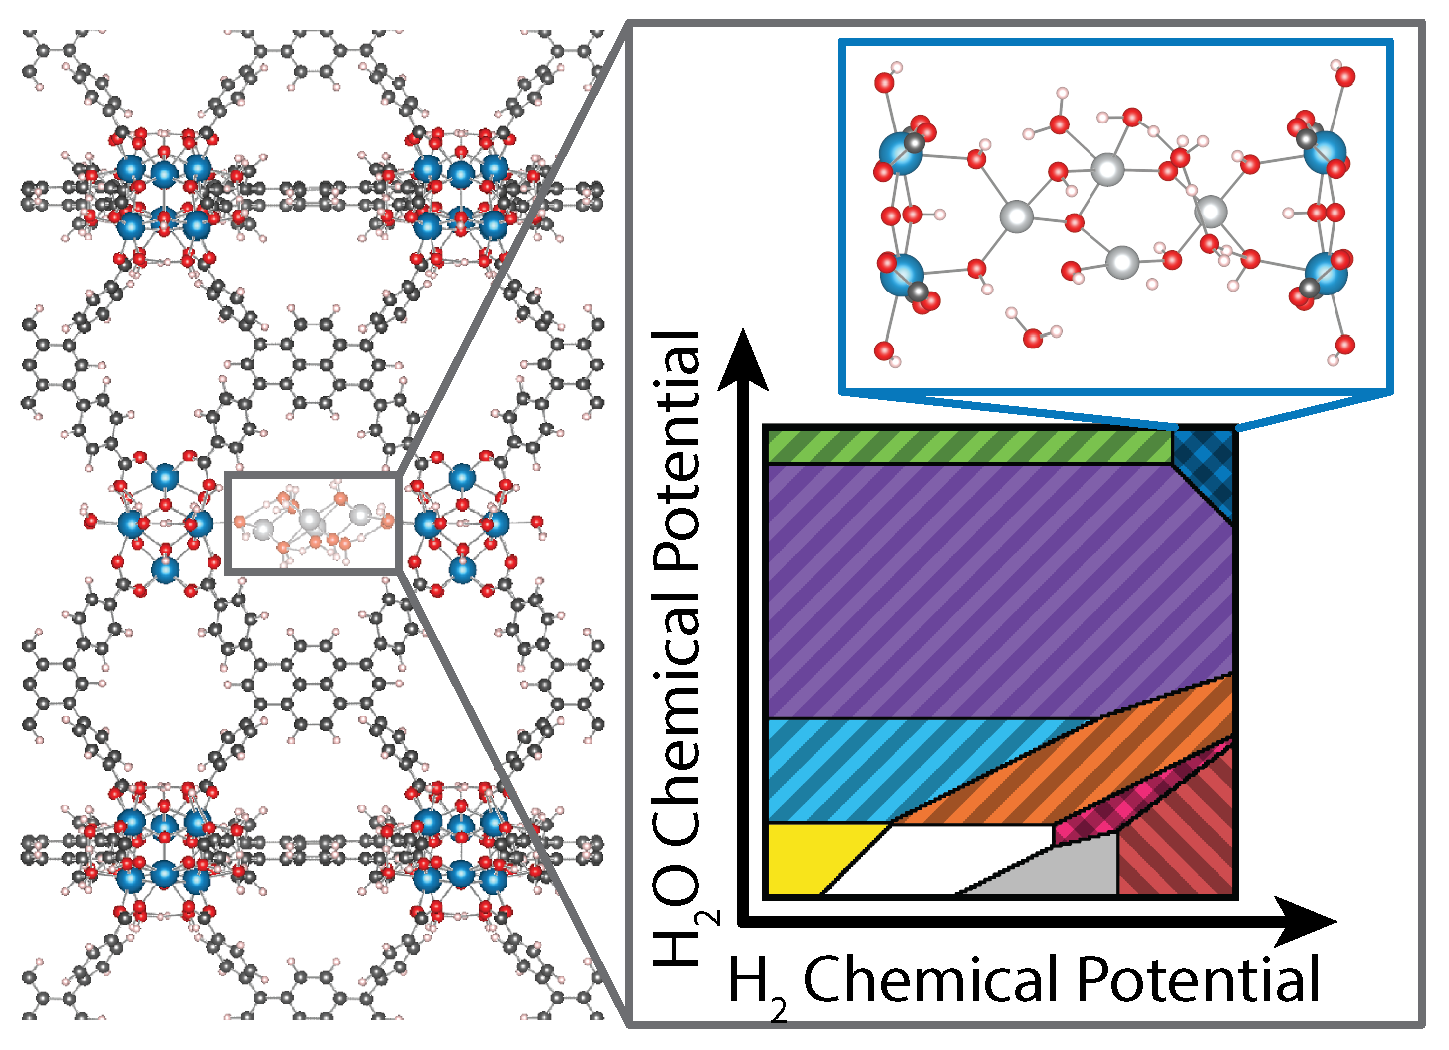
\includegraphics{zi-images/00-General-Graphics/2022-figure-TOC.png}
\end{figure}

\end{document}
